\documentclass[aspectratio=169,10pt]{beamer}

% ===================== NGÔN NGỮ & PHÔNG CHỮ (pdfLaTeX — Latin Modern Sans T5) =====================
\usepackage[utf8]{inputenc}
\usepackage[T5]{fontenc}
\usepackage{lmodern}
\usepackage[vietnamese,provide=*]{babel}

% ===================== GÓI HỖ TRỢ =====================
\usepackage{amsmath,amssymb}
\usepackage{graphicx}
\graphicspath{{../Report/figures/}}
\usepackage{booktabs}
\usepackage{tabularx}
\usepackage{array}
\usepackage{colortbl}
\usepackage{xcolor}
\usepackage{tikz}
\usetikzlibrary{arrows.meta,positioning,shapes.geometric}
\usepackage{tcolorbox}
\usepackage{listings}

% ===================== BẢNG MÀU ĐỒNG BỘ: XANH LAM ĐẬM & TRẮNG =====================
\definecolor{BlueDark}{RGB}{11,53,104}      % Xanh lam đậm chủ đạo
\definecolor{BlueMid}{RGB}{24,92,162}       % Xanh lam trung bình (nhấn đồng bộ)
\definecolor{BlueSoft}{RGB}{238,244,251}    % Xanh lam rất nhạt cho nền thân hộp / bảng
\definecolor{BlueBorder}{RGB}{188,210,234}  % Viền xanh lam dịu
\definecolor{Ink}{RGB}{22,36,54}            % Chữ chính đậm dễ đọc
\definecolor{Muted}{RGB}{88,108,132}        % Chữ phụ / chú thích
% Màu ngữ nghĩa nhẹ chỉ dùng cho con số trong bảng kết quả
\definecolor{OkGreen}{RGB}{21,128,61}
\definecolor{BadRed}{RGB}{190,32,48}
\definecolor{WarnAmber}{RGB}{180,98,6}

% ===================== CẤU HÌNH BEAMER =====================
\usetheme{default}
\setbeamertemplate{navigation symbols}{}
\setbeamersize{text margin left=0.55cm, text margin right=0.55cm}

\setbeamercolor{normal text}{fg=Ink,bg=white}
\setbeamercolor{structure}{fg=BlueDark}
\setbeamercolor{frametitle}{fg=white,bg=BlueDark}
\setbeamercolor{itemize item}{fg=BlueMid}
\setbeamercolor{itemize subitem}{fg=BlueDark}
\setbeamercolor{enumerate item}{fg=BlueDark}
\setbeamertemplate{itemize item}{\raisebox{0.15ex}{\tiny$\blacksquare$}}
\setbeamertemplate{itemize subitem}{\raisebox{0.1ex}{\scriptsize$\blacktriangleright$}}

% Nhãn phần & người thuyết trình trên thanh tiêu đề & chân trang
\newcommand{\currentpart}{Mở đầu}
\newcommand{\setpart}[1]{\renewcommand{\currentpart}{#1}}

% Thanh tiêu đề nền Xanh lam đậm + chữ trắng sắc nét
\setbeamercolor{frametitle rule}{bg=BlueMid}
\setbeamertemplate{frametitle}{%
  \nointerlineskip
  \begin{beamercolorbox}[wd=\paperwidth,ht=0.84cm,dp=0.26cm,leftskip=0.55cm,rightskip=0.55cm]{frametitle}%
    \makebox[\dimexpr\paperwidth-1.1cm\relax][s]{%
      {\bfseries\normalsize\color{white}\insertframetitle}\hfill
      {\scriptsize\color{white!82}\currentpart}%
    }%
  \end{beamercolorbox}%
  \nointerlineskip
  \begin{beamercolorbox}[wd=\paperwidth,ht=1.8pt,dp=0pt]{frametitle rule}\end{beamercolorbox}%
  \vspace{-0.12cm}
}

% Chân trang nền trắng tối giản + thanh tiến trình xanh lam
\setbeamertemplate{footline}{%
  \leavevmode%
  \begin{tikzpicture}[remember picture,overlay]
    \fill[BlueBorder] (current page.south west) rectangle ([yshift=2.2pt]current page.south east);
    \pgfmathsetmacro{\prog}{\insertframenumber/\inserttotalframenumber}
    \fill[BlueDark] (current page.south west) rectangle ([xshift=\prog\paperwidth,yshift=2.2pt]current page.south west);
  \end{tikzpicture}%
  \hbox{%
    \begin{beamercolorbox}[wd=0.56\paperwidth,ht=2.0ex,dp=1.1ex,leftskip=0.55cm]{author in head/foot}%
      \tiny\color{Muted}Đánh giá mã C++ hiện đại \& MPI+OpenMP do LLM sinh --- HUS
    \end{beamercolorbox}%
    \begin{beamercolorbox}[wd=0.32\paperwidth,ht=2.0ex,dp=1.1ex,center]{title in head/foot}%
      \tiny\color{BlueMid}\currentpart
    \end{beamercolorbox}%
    \begin{beamercolorbox}[wd=0.12\paperwidth,ht=2.0ex,dp=1.1ex,right,rightskip=0.55cm]{date in head/foot}%
      \tiny\bfseries\color{BlueDark}\insertframenumber\,/\,\inserttotalframenumber
    \end{beamercolorbox}%
  }%
  \vskip1.5pt%
}

% ===================== HỆ THỐNG KHỐI HỘP ĐỒNG BỘ 100% =====================
% Kiểu chính: thanh tiêu đề xanh lam đậm chữ trắng + thân xanh nhạt/trắng (giống mẫu "Luật chơi")
\newtcolorbox{bluebox}[2][]{
  colback=BlueSoft, colframe=BlueDark, colbacktitle=BlueDark, coltitle=white,
  boxrule=0.55pt, arc=2pt,
  before skip=0pt, after skip=0pt,
  left=6pt, right=6pt, top=3.5pt, bottom=3.5pt,
  toptitle=2.2pt, bottomtitle=2.2pt, boxsep=0.5pt,
  fonttitle=\bfseries\footnotesize, title={#2},
  before upper={\raggedright}, #1
}
% Kiểu phụ nhấn nhẹ: cùng hình dáng, thanh tiêu đề xanh lam trung bình (BlueMid)
\newtcolorbox{hboxcard}[2][]{
  colback=white, colframe=BlueMid, colbacktitle=BlueMid, coltitle=white,
  boxrule=0.55pt, arc=2pt,
  before skip=0pt, after skip=0pt,
  left=6pt, right=6pt, top=3.5pt, bottom=3.5pt,
  toptitle=2.2pt, bottomtitle=2.2pt, boxsep=0.5pt,
  fonttitle=\bfseries\footnotesize, title={#2},
  before upper={\raggedright}, #1
}
% Hộp gọn không tiêu đề (chỉ dùng cho chú thích ngắn) — đồng bộ viền & màu
\newtcolorbox{plainbox}[1][]{
  colback=BlueSoft, colframe=BlueBorder, leftrule=2.5pt,
  boxrule=0.55pt, arc=2pt,
  before skip=0pt, after skip=0pt,
  left=6pt, right=6pt, top=3.5pt, bottom=3.5pt, boxsep=0.5pt,
  before upper={\raggedright}, #1
}

% ===================== MÃ NGUỒN =====================
\lstset{
  language=C++,
  basicstyle=\ttfamily\scriptsize,
  keywordstyle=\color{BlueDark}\bfseries,
  commentstyle=\color{Muted}\itshape,
  stringstyle=\color{BlueMid},
  breaklines=true,
  columns=fullflexible,
  keepspaces=true,
  showstringspaces=false,
  tabsize=2,
  aboveskip=1.5pt,
  belowskip=1.5pt
}

% ===================== LỆNH TIỆN ÍCH =====================
\newcommand{\code}[1]{\texttt{\color{BlueDark}#1}}
\newcommand{\ok}[1]{\textcolor{OkGreen}{\bfseries #1}}
\newcommand{\bad}[1]{\textcolor{BadRed}{\bfseries #1}}
\newcommand{\warn}[1]{\textcolor{WarnAmber}{\bfseries #1}}
\newcommand{\pill}[1]{%
  \tikz[baseline=(X.base)]\node[fill=white,text=BlueDark,rounded corners=1.5pt,inner xsep=4pt,inner ysep=0.8pt,font=\tiny\bfseries](X){#1};%
}

% ==========================================================================
\begin{document}

% ==========================================================================
% SLIDE 1: TRANG BÌA (XANH LAM ĐẬM + TRẮNG)
% ==========================================================================
\begin{frame}[plain]
\begin{tikzpicture}[remember picture,overlay]
  % Nền trên màu xanh lam đậm
  \fill[BlueDark] (current page.north west) rectangle ([yshift=-4.40cm]current page.north east);
  \fill[BlueMid] ([yshift=-4.40cm]current page.north west) rectangle ([yshift=-4.54cm]current page.north east);
  \fill[BlueMid,opacity=0.25] ([xshift=-3.8cm]current page.north east) -- (current page.north east) -- ([yshift=-4.40cm]current page.north east) -- cycle;

  % Logo trường góc trên trái
  \node[anchor=north west] at ([xshift=0.70cm,yshift=-0.35cm]current page.north west) {%
    \begin{tcolorbox}[width=1.28cm,colback=white,colframe=white,arc=3pt,boxsep=1.5pt,left=1.5pt,right=1.5pt,top=1.5pt,bottom=1.5pt]
      \centering
\includegraphics[width=1.02cm]{logo.png}
    \end{tcolorbox}
  };
  % Đơn vị học thuật
  \node[anchor=north west,text=white] at ([xshift=2.22cm,yshift=-0.46cm]current page.north west) {%
    \begin{minipage}{12cm}
      {\footnotesize\color{white!82}TRƯỜNG ĐẠI HỌC KHOA HỌC TỰ NHIÊN --- KHOA TOÁN -- CƠ -- TIN HỌC}\\[2pt]
      {\small\bfseries\color{BlueSoft}BÁO CÁO BỘ MÔN TÍNH TOÁN SONG SONG}
    \end{minipage}
  };
  % Tiêu đề chính
  \node[anchor=north west,text=white] at ([xshift=0.70cm,yshift=-2.18cm]current page.north west) {%
    \begin{minipage}{14.6cm}
      {\large\bfseries ĐÁNH GIÁ MÃ C++ HIỆN ĐẠI VÀ MPI+OPENMP DO LLM SINH\\[2pt]
      CHO BÀI TOÁN TẬP MANDELBROT CÓ KHẢ NĂNG MỞ RỘNG}\\[5pt]
      {\footnotesize\itshape\color{white!82}Evaluating LLM-Generated Modern C++ and MPI+OpenMP Codes for Scalable Mandelbrot Set Computation}
    \end{minipage}
  };
  % Nửa dưới nền trắng: thành viên & GVHD (đồng bộ 1 kiểu khung xanh lam)
  \node[anchor=north west] at ([xshift=0.70cm,yshift=-4.88cm]current page.north west) {%
    \begin{minipage}{14.6cm}
      \begin{columns}[T,totalwidth=14.6cm]
        \begin{column}{0.66\textwidth}
          {\scriptsize\bfseries\color{BlueDark}SINH VIÊN THỰC HIỆN}\par\vspace{5pt}
          \noindent
          \begin{minipage}[t]{0.485\textwidth}
            \begin{tcolorbox}[colback=BlueSoft,colframe=BlueDark,leftrule=2.6pt,boxrule=0.5pt,arc=2pt,before skip=0pt,after skip=0pt,height=1.20cm,valign=center,left=6pt,right=5pt,top=2pt,bottom=2pt,boxsep=1pt]
              {\small\bfseries\color{BlueDark}Nguyễn Quang Anh}\\[-1pt]
              {\scriptsize\color{Muted}24001649 \;\textbullet\; \textcolor{BlueMid}{\bfseries Nhóm trưởng}}
            \end{tcolorbox}
            \vspace{0.24cm}
            \begin{tcolorbox}[colback=BlueSoft,colframe=BlueMid,leftrule=2.6pt,boxrule=0.5pt,arc=2pt,before skip=0pt,after skip=0pt,height=1.20cm,valign=center,left=6pt,right=5pt,top=2pt,bottom=2pt,boxsep=1pt]
              {\small\bfseries\color{BlueDark}Đồng Đức Dương}\\[-1pt]
              {\scriptsize\color{Muted}24001659 \;\textbullet\; Thành viên}
            \end{tcolorbox}
          \end{minipage}\hfill
          \begin{minipage}[t]{0.485\textwidth}
            \begin{tcolorbox}[colback=BlueSoft,colframe=BlueMid,leftrule=2.6pt,boxrule=0.5pt,arc=2pt,before skip=0pt,after skip=0pt,height=1.20cm,valign=center,left=6pt,right=5pt,top=2pt,bottom=2pt,boxsep=1pt]
              {\small\bfseries\color{BlueDark}Nguyễn Như Bảo}\\[-1pt]
              {\scriptsize\color{Muted}24001655 \;\textbullet\; Thành viên}
            \end{tcolorbox}
            \vspace{0.24cm}
            \begin{tcolorbox}[colback=BlueSoft,colframe=BlueMid,leftrule=2.6pt,boxrule=0.5pt,arc=2pt,before skip=0pt,after skip=0pt,height=1.20cm,valign=center,left=6pt,right=5pt,top=2pt,bottom=2pt,boxsep=1pt]
              {\small\bfseries\color{BlueDark}Trần Lý Dũng}\\[-1pt]
              {\scriptsize\color{Muted}24001658 \;\textbullet\; Thành viên}
            \end{tcolorbox}
          \end{minipage}
        \end{column}
        \begin{column}{0.32\textwidth}
          {\scriptsize\bfseries\color{BlueDark}GIẢNG VIÊN HƯỚNG DẪN}\par\vspace{5pt}
          \begin{tcolorbox}[colback=BlueSoft,colframe=BlueDark,leftrule=2.6pt,boxrule=0.5pt,arc=2pt,before skip=0pt,after skip=0pt,height=2.64cm,valign=center,left=7pt,right=6pt,top=3pt,bottom=3pt,boxsep=1pt]
            {\small\bfseries\color{BlueDark}TS. Nguyễn Hải Vinh}\\[2pt]
            {\small\bfseries\color{BlueDark}TS. Mạc Đăng Trường}\\[7pt]
            {\scriptsize\color{Muted}Bài báo gốc: Diehl, Nader \& Gupta\\(arXiv:2512.17023v2)}\\[4pt]
            {\scriptsize\bfseries\color{BlueMid}Hà Nội, 11/2026}
          \end{tcolorbox}
        \end{column}
      \end{columns}
    \end{minipage}
  };
\end{tikzpicture}
\end{frame}

% ==========================================================================
% SLIDE 2: BỐ CỤC 4 PHẦN THUYẾT TRÌNH
% ==========================================================================
\setpart{Mở đầu \textbullet{} Bố cục}
\begin{frame}{Bố cục 4 phần thuyết trình}
\begin{columns}[T,totalwidth=\textwidth]
  \begin{column}{0.485\textwidth}
    \begin{bluebox}[height=2.95cm]{Phần 1 \;\textbullet\; Giới thiệu bài toán \hfill {\scriptsize Slide 3--5}}
      \textbf{\footnotesize Trần Lý Dũng} {\scriptsize(\color{Muted}24001658)}
      \begin{itemize}\scriptsize\setlength{\itemsep}{2pt}
        \item Bối cảnh HPC--LLM \& 3 khoảng trống nghiên cứu.
        \item Mục tiêu, 3 câu hỏi RQ1--RQ3 \& các đóng góp chính.
        \item Bài toán tập Mandelbrot, mất cân bằng tải \& định dạng Netpbm.
      \end{itemize}
    \end{bluebox}
  \end{column}
  \begin{column}{0.485\textwidth}
    \begin{bluebox}[height=2.95cm]{Phần 2 \;\textbullet\; Thực nghiệm \& Demo \hfill {\scriptsize Slide 6--11}}
      \textbf{\footnotesize Nguyễn Quang Anh} {\scriptsize(\color{Muted}24001649 --- Nhóm trưởng)}
      \begin{itemize}\scriptsize\setlength{\itemsep}{2pt}
        \item Tiến hóa C++11/17/20 \& 5 mô hình song song đánh giá.
        \item Ma trận 4 LLM $\times$ 5 biến thể, \code{rostam} \& bộ prompt P1--P3.
        \item Quy trình 4 cổng, độ đo \code{px/s} \& \textbf{Demo trực tiếp} (lỗi \code{-t}).
      \end{itemize}
    \end{bluebox}
  \end{column}
\end{columns}

\vspace{0.28cm}

\begin{columns}[T,totalwidth=\textwidth]
  \begin{column}{0.485\textwidth}
    \begin{bluebox}[height=2.95cm]{Phần 3 \;\textbullet\; Phân tích lỗi thực tế \hfill {\scriptsize Slide 12--16}}
      \textbf{\footnotesize Đồng Đức Dương} {\scriptsize(\color{Muted}24001659)}
      \begin{itemize}\scriptsize\setlength{\itemsep}{2pt}
        \item Hố ngăn cách giữa Biên dịch (100\%) và Thực thi.
        \item 4 nhóm lỗi tiêu biểu (TBB, Coroutine, P4/P5, MPI).
        \item Phân tầng lỗi, kích thước LOC \& mô hình COCOMO.
      \end{itemize}
    \end{bluebox}
  \end{column}
  \begin{column}{0.485\textwidth}
    \begin{bluebox}[height=2.95cm]{Phần 4 \;\textbullet\; Hiệu năng \& tổng kết \hfill {\scriptsize Slide 17--22}}
      \textbf{\footnotesize Nguyễn Như Bảo} {\scriptsize(\color{Muted}24001655)}
      \begin{itemize}\scriptsize\setlength{\itemsep}{2pt}
        \item Mở rộng 1 nút (1--20 lõi), phân tán (1--12 nút) \& \code{Human [5]}.
        \item \textbf{Bổ sung thực nghiệm:} kiểm chứng Gemini 4 Hydrogen.
        \item 5 khuyến nghị thực hành, danh mục kiểm duyệt \& Q\&A.
      \end{itemize}
    \end{bluebox}
  \end{column}
\end{columns}
\end{frame}

% ==========================================================================
% PHẦN 1: GIỚI THIỆU BÀI TOÁN (TRẦN LÝ DŨNG)
% ==========================================================================
\setpart{Phần 1 \textbullet{} Trần Lý Dũng}

% SLIDE 3: BỐI CẢNH & VẤN ĐỀ NGHIÊN CỨU
\begin{frame}{Bối cảnh \& Vấn đề nghiên cứu}
\begin{columns}[T,totalwidth=\textwidth]
  \begin{column}{0.485\textwidth}
    \begin{bluebox}[height=5.76cm]{Bối cảnh: HPC hiện đại \& LLM sinh mã}
      \begin{itemize}\scriptsize\setlength{\itemsep}{4.5pt}
        \item \textbf{Hai trụ cột song song HPC:} \emph{bộ nhớ chia sẻ} (nhiều luồng chung RAM --- chi phí đồng bộ/tranh chấp) và \emph{bộ nhớ phân tán} (nhiều nút trao đổi thông điệp --- chi phí độ trễ/băng thông).
        \item \textbf{Đa dạng cơ chế, mở rộng không gian lỗi:} C++11/17/20, OpenMP và MPI cùng tồn tại; mã biên dịch sạch vẫn có thể sai kết quả hoặc không tận dụng đủ số lõi.
        \item \textbf{Thách thức với LLM:} các đánh giá trước chủ yếu xét mã tuần tự; mã HPC đòi hỏi đồng thời tính đúng, tương thích \emph{toolchain}, kiểm soát tài nguyên và mở rộng trên phần cứng thật.
      \end{itemize}
    \end{bluebox}
  \end{column}
  \begin{column}{0.485\textwidth}
    \begin{hboxcard}[height=3.62cm]{Vấn đề \& 3 khoảng trống nghiên cứu}
      \begin{enumerate}\scriptsize\setlength{\itemsep}{3.5pt}
        \item \textbf{Đánh giá đơn mô hình:} nghiên cứu trước thường chỉ xét riêng OpenMP, OpenACC hoặc MPI --- thiếu so sánh ngang hàng giữa các mức trừu tượng.
        \item \textbf{Chưa đo mở rộng thực tế:} phần lớn dừng ở tỉ lệ biên dịch hoặc vượt test, chưa đo \emph{scaling} trên cụm HPC thật.
        \item \textbf{Bỏ ngỏ hệ sinh thái công cụ:} hiếm khi kiểm chứng hiểu biết của LLM về trình biên dịch, backend thư viện và chuẩn C++.
      \end{enumerate}
    \end{hboxcard}
    \vspace{0.22cm}
    \begin{bluebox}[height=1.92cm]{Vì sao chọn Mandelbrot làm phép thử?}
      \scriptsize Là \textbf{benchmark tối thiểu có kiểm soát} (\emph{song song hiển nhiên}, không cần bộ giải ngoài) $\implies$ cô lập thuần năng lực sinh mã song song, quản lý luồng và xuất kết quả của LLM.
    \end{bluebox}
  \end{column}
\end{columns}
\end{frame}

% SLIDE 4: MỤC TIÊU, 3 CÂU HỎI RQ & ĐÓNG GÓP
\begin{frame}{Mục tiêu, Câu hỏi nghiên cứu \& Đóng góp}
\begin{columns}[T,totalwidth=\textwidth]
  \begin{column}{0.485\textwidth}
    \begin{bluebox}[height=1.74cm,top=3pt,bottom=3pt]{Mục tiêu đánh giá (\emph{ảnh chụp thời điểm})}
      \scriptsize Đánh giá có hệ thống \textbf{4 LLM} (ChatGPT-4, ChatGPT-5, Claude, LLaMA) trên \textbf{5 biến thể}: C++11 \code{async}, C++17 \code{par\_algo}, C++20 coroutine, OpenMP và MPI+OpenMP.
    \end{bluebox}
    \vspace{0.20cm}
    \begin{hboxcard}[height=4.20cm,top=4pt,bottom=4pt]{Ba câu hỏi nghiên cứu (RQ1 -- RQ3)}
      \begin{itemize}\scriptsize\setlength{\itemsep}{5pt}
        \item \textbf{RQ1 (Biên dịch):} LLM sinh mã C++ song song đúng cú pháp và biên dịch được ở mức nào?
        \item \textbf{RQ2 (Lỗi thực thi \& ngữ nghĩa):} Những lỗi nào xuất hiện, mức độ khó sửa đến đâu và nguyên nhân gốc là gì?
        \item \textbf{RQ3 (Mở rộng \& so sánh):} Sau khi sửa tối thiểu, mã có mở rộng theo số lõi/nút và cạnh tranh được với mã con người viết không?
      \end{itemize}
    \end{hboxcard}
  \end{column}
  \begin{column}{0.485\textwidth}
    \begin{bluebox}[height=3.34cm,top=3pt,bottom=3pt]{Đóng góp của bài báo gốc (4 điểm)}
      \begin{enumerate}\scriptsize\setlength{\itemsep}{1.8pt}
        \item Thiết kế bộ prompt nhất quán cho C++11/17/20, OpenMP và MPI+OpenMP.
        \item Phân tích chi tiết biên dịch, lỗi thực thi và tính đúng chức năng.
        \item Đánh giá \textbf{C++20 coroutine} --- cơ chế mới đang tích hợp vào Kokkos, HPX.
        \item Phân loại lỗi, cách khắc phục và chỉ ra giới hạn LLM trong gỡ lỗi HPC.
      \end{enumerate}
    \end{bluebox}
    \vspace{0.20cm}
    \begin{hboxcard}[height=2.60cm,top=3pt,bottom=3pt]{Đóng góp mở rộng của báo cáo nhóm (3 điểm)}
      \begin{itemize}\scriptsize\setlength{\itemsep}{1.8pt}
        \item Hệ thống hóa lý thuyết từng mô hình, lý giải \textbf{nguyên nhân gốc} gây lỗi.
        \item Xây dựng bảng phân tầng lỗi theo 6 lớp kèm mức khó sửa.
        \item Chuyển thành quy trình \& danh mục kiểm duyệt thực dụng (kèm demo \& Gemini 4).
      \end{itemize}
    \end{hboxcard}
  \end{column}
\end{columns}
\end{frame}

% SLIDE 4: BÀI TOÁN TẬP MANDELBROT
\begin{frame}{Bài toán tập Mandelbrot \& tính mất cân bằng tải}
\begin{columns}[T,totalwidth=\textwidth]
  \begin{column}{0.50\textwidth}
    \begin{bluebox}{Định nghĩa thuật toán thoát (\emph{escape-time})}
      \centering $z_0 = 0, \qquad z_{k+1} = z_k^2 + c \quad (c = c_r + i c_i)$\\[4pt]
      \raggedright\scriptsize Dừng khi $|z_k| > 2$ (ngoài tập) hoặc chạm $I_{\max} = 1000$ vòng (trong tập --- vùng đen đặc).
    \end{bluebox}
    \vspace{0.22cm}
    \begin{hboxcard}{Đặc trưng tính toán \& định dạng đầu ra}
      \begin{itemize}\scriptsize\setlength{\itemsep}{2.5pt}
        \item \textbf{Song song hiển nhiên (\emph{embarrassingly parallel}):} mỗi điểm ảnh độc lập hoàn toàn, không cần thư viện giải toán ngoài.
        \item \textbf{Mất cân bằng tải tự nhiên:} nền trắng thoát sau 1--3 vòng; ruột đen chạy đủ 1000 vòng $\implies$ chia tĩnh (\code{static}) gây nghẽn tải nặng!
        \item \textbf{Định dạng Netpbm (PBM/PGM):} tối giản, nhưng dễ nhầm \code{P4} (1 bit/px) với \code{P5} (1 byte/px).
      \end{itemize}
    \end{hboxcard}
  \end{column}
  \begin{column}{0.47\textwidth}
    \centering
    
\includegraphics[width=0.77\linewidth]{mandelbrot_coroutine.png}\\[-2pt]
    {\tiny\color{Muted}(a) ChatGPT-5 --- C++20 Coroutines ($1920\times 1080$)}\\[3pt]
    
\includegraphics[width=0.77\linewidth]{mandelbrot_mpi.jpg}\\[-2pt]
    {\tiny\color{Muted}(b) ChatGPT-5 --- MPI+OpenMP (khác bảng màu dù cùng LLM!)}
  \end{column}
\end{columns}
\end{frame}

% ==========================================================================
% PHẦN 2: 5 MÔ HÌNH SONG SONG, KIẾN TRÚC THỰC NGHIỆM & DEMO (NGUYỄN QUANG ANH)
% ==========================================================================
\setpart{Phần 2 \textbullet{} Nguyễn Quang Anh}

% SLIDE 5: TIẾN HÓA SONG SONG TRONG C++ HIỆN ĐẠI
\begin{frame}{Tiến hóa lập trình song song trong chuẩn C++ hiện đại}
\centering
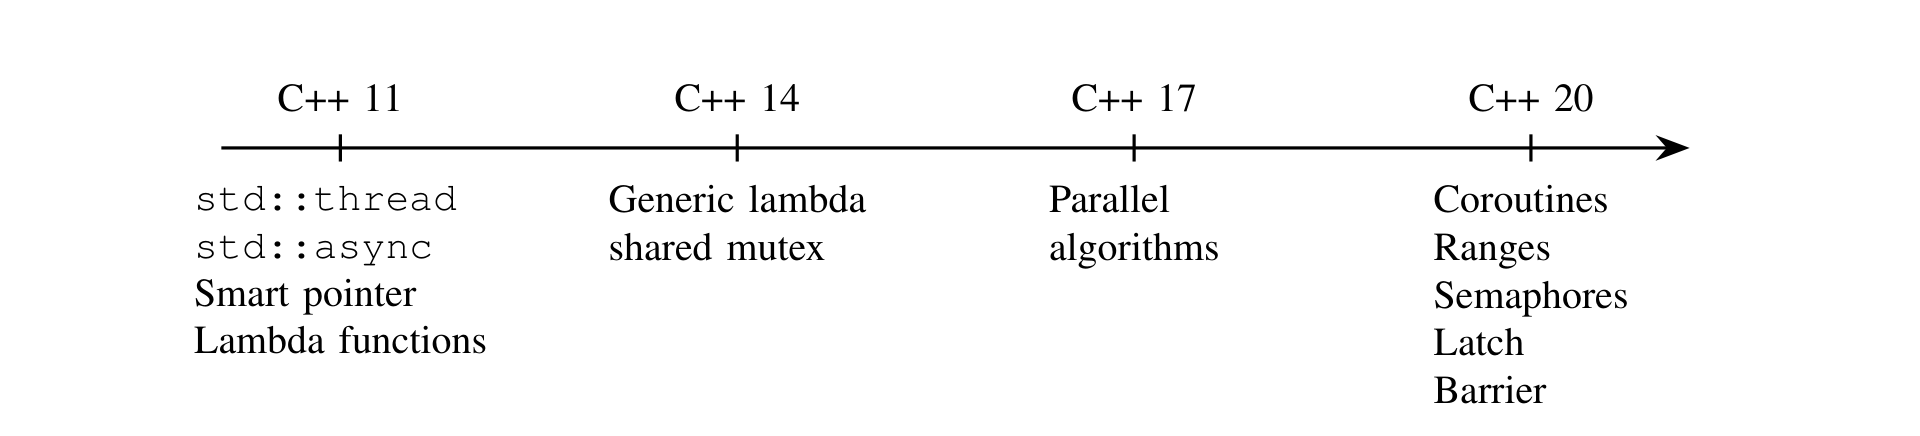
\includegraphics[width=0.92\textwidth]{fig_timeline.png}\\[-2pt]
{\scriptsize\color{Muted}Hình 2: Dòng thời gian các tính năng song song bổ sung vào chuẩn C++ (Nguồn: Diehl et al., phỏng theo chuẩn ISO C++).}

\vspace{0.25cm}
\begin{columns}[T,totalwidth=\textwidth]
  \begin{column}{0.32\textwidth}
    \begin{bluebox}[height=2.25cm]{C++11 \;\textbullet\; Bất đồng bộ}
      \scriptsize \code{std::thread}, \code{std::async}, \code{std::future}. Phổ biến lâu đời, nhiều mã mẫu trên mạng $\implies$ LLM quen thuộc nhất.
    \end{bluebox}
  \end{column}
  \begin{column}{0.32\textwidth}
    \begin{bluebox}[height=2.25cm]{C++17 \;\textbullet\; Thuật toán song song}
      \scriptsize \code{std::execution::par} viết ngắn gọn nhưng \textbf{ẩn backend}: trên GCC/Linux dùng \textbf{Intel TBB}, không dùng OpenMP!
    \end{bluebox}
  \end{column}
  \begin{column}{0.32\textwidth}
    \begin{bluebox}[height=2.25cm]{C++20 \;\textbullet\; Coroutines}
      \scriptsize \code{co\_await}, \code{co\_return}, \code{promise\_type}, \code{std::latch}. Mới, ít ví dụ chuẩn, đòi hỏi kiểm soát chặt vòng đời frame.
    \end{bluebox}
  \end{column}
\end{columns}
\end{frame}

% SLIDE 6: 5 MÔ HÌNH SONG SONG ĐƯỢC ĐÁNH GIÁ
\begin{frame}{Tổng quan 5 mô hình lập trình song song được đánh giá}
\begin{bluebox}[top=8pt,bottom=8pt]{So sánh 5 biến thể: 4 bộ nhớ chia sẻ (1 nút) + 1 phân tán (N nút) --- Bảng 2}
  \footnotesize
  \renewcommand{\arraystretch}{1.52}
  \begin{tabularx}{\textwidth}{@{}>{\bfseries\color{BlueDark}}l l >{\raggedright\arraybackslash}p{4.35cm} >{\raggedright\arraybackslash}X@{}}
    \toprule
    \textbf{Biến thể} & \textbf{Bộ nhớ} & \textbf{Điều khiển luồng / phân vùng} & \textbf{Điểm dễ sai đối với LLM} \\
    \midrule
    C++11 \code{std::async} & Chia sẻ (1 nút) & Chia $T$ tác vụ theo cờ \code{-t} & Quên \code{launch::async}; chia tĩnh lệch tải \\
    C++17 \code{par\_algo} & Chia sẻ (1 nút) & Backend \code{tbb::global\_control} & Nhầm OpenMP (\code{OMP\_NUM\_THREADS} vô tác dụng) \\
    C++20 Coroutines & Chia sẻ (1 nút) & Quản lý handle, \code{promise\_type}, pool & Treo vòng \code{done()}; \emph{double-free} / segfault \\
    OpenMP & Chia sẻ (1 nút) & \code{\#pragma omp parallel for} + \code{-t} & Bỏ qua cờ \code{-t} hoặc lập lịch \code{static} kém \\
    \midrule
    MPI + OpenMP & \textcolor{BlueMid}{\bfseries Phân tán (N nút)} & Chia phân vùng theo \code{-p} + OpenMP nội bộ & Mọi rank tính cả ảnh; sai \code{MPI\_Gather}; thiếu đo truyền thông \\
    \bottomrule
  \end{tabularx}
\end{bluebox}
\end{frame}

% SLIDE 7: MA TRẬN THỰC NGHIỆM & HẠ TẦNG ĐO
\begin{frame}{Ma trận thực nghiệm (4 LLM $\times$ 5 biến thể) \& Hạ tầng đo}
\begin{columns}[T,totalwidth=\textwidth]
  \begin{column}{0.485\textwidth}
    \begin{bluebox}[height=3.65cm]{Ma trận 20 chương trình (Bảng 4)}
      \centering
      \scriptsize
      \renewcommand{\arraystretch}{1.24}
      \begin{tabular}{@{}lcccc@{}}
        \toprule
        \textbf{Biến thể} & \textbf{GPT-5} & \textbf{GPT-4} & \textbf{Claude} & \textbf{LLaMA} \\
        \midrule
        C++11 \code{async}     & \ok{\checkmark} & \ok{\checkmark} & \ok{\checkmark} & \ok{\checkmark} \\
        C++17 \code{par\_algo} & \ok{\checkmark} & \ok{\checkmark} & \ok{\checkmark} & \ok{\checkmark} \\
        C++20 \code{coroutine} & \ok{\checkmark} & \ok{\checkmark} & \ok{\checkmark} & \ok{\checkmark} \\
        OpenMP                 & \ok{\checkmark} & \ok{\checkmark} & \ok{\checkmark} & \ok{\checkmark} \\
        MPI + OpenMP           & \ok{\checkmark} & \ok{\checkmark} & \ok{\checkmark} & \ok{\checkmark} \\
        \bottomrule
      \end{tabular}
    \end{bluebox}
    \vspace{0.22cm}
    \begin{hboxcard}[height=1.72cm]{Nguyên tắc sinh mã}
      \scriptsize Mỗi cặp (LLM, biến thể) gửi prompt \textbf{1 lần duy nhất}, không kèm ngữ cảnh hay gợi ý sửa lỗi; con người chỉ sửa tối thiểu sau khi ghi nhận đầy đủ lỗi.
    \end{hboxcard}
  \end{column}
  \begin{column}{0.485\textwidth}
    \begin{bluebox}[height=3.65cm]{Cụm HPC \texttt{rostam} --- ĐH LSU (Bảng 5)}
      \begin{itemize}\scriptsize\setlength{\itemsep}{2.5pt}
        \item \textbf{Phần cứng:} phân vùng \code{medusa}, 16 nút; mỗi nút 1 CPU Intel Xeon Gold 6148 (\textbf{20 lõi}, 2.40\,GHz), 92\,GB RAM.
        \item \textbf{Toolchain:} GCC 11.5.0, Intel TBB 2022.2, OpenMPI 5.0.7.
        \item \textbf{Đo 1 nút:} quét \code{1 $\to$ 20} lõi (4 biến thể chia sẻ).
        \item \textbf{Đo phân tán:} ảnh $12000\times 80000$, 1000 vòng, \code{1, 2, 4, 8, 12} nút (1 rank MPI $\times$ 20 lõi OpenMP/nút).
      \end{itemize}
    \end{bluebox}
    \vspace{0.22cm}
    \begin{hboxcard}[height=1.72cm]{Mốc so sánh con người (\texttt{Human [5]})}
      \scriptsize 5 chương trình C++ chạy thật từ sách \emph{Parallel C++} (Diehl et al., 2024) biên dịch và đo trên cùng cụm \code{rostam}.
    \end{hboxcard}
  \end{column}
\end{columns}
\end{frame}

% SLIDE 8: THIẾT KẾ BỘ PROMPT P1, P2, P3
\begin{frame}{Thiết kế bộ prompt nguyên văn P1, P2, P3}
\begin{bluebox}[top=2.5pt,bottom=2.5pt,toptitle=1.6pt,bottomtitle=1.6pt]{\pill{P1} \; C++ hiện đại (C++11 async / C++17 par\_algo / C++20 coroutines)}
  \scriptsize\ttfamily "Write a parallel code for the Mandelbrot set using C++ \{11 async future, 17 parallel algorithms, 20 coroutines\} and write the output to the PBM format. Make the number of threads configurable with the command line option -t and print the runtime excluding IO."
\end{bluebox}
\vspace{0.18cm}
\begin{bluebox}[top=2.5pt,bottom=2.5pt,toptitle=1.6pt,bottomtitle=1.6pt]{\pill{P2} \; OpenMP (Bộ nhớ chia sẻ)}
  \scriptsize\ttfamily "Write a parallel code for the Mandelbrot set using C++ using OpenMP and write the output to the PBM format. Make the number of threads configurable with the command line option -t and print the runtime excluding IO."
\end{bluebox}
\vspace{0.18cm}
\begin{bluebox}[top=2.5pt,bottom=2.5pt,toptitle=1.6pt,bottomtitle=1.6pt]{\pill{P3} \; MPI + OpenMP (Bộ nhớ phân tán)}
  \scriptsize\ttfamily "Write a distributed code using MPI for the Mandelbrot set and using OpenMP for parallelism in C++ and write the output to the PBM format. Make the number of partitions configurable with the command line option -p and print the runtime excluding IO."
\end{bluebox}
\vspace{0.18cm}
\begin{hboxcard}[top=2.5pt,bottom=2.5pt,toptitle=1.6pt,bottomtitle=1.6pt]{Hai lưu ý quan trọng về thiết kế prompt}
  \scriptsize
  \textbf{1. Bắt buộc thêm \code{-p} ở P3:} nếu không yêu cầu số phân vùng, LLM sinh mã để \emph{mọi rank MPI tự tính lại nguyên cả bức ảnh}!\\[1pt]
  \textbf{2. Không cố định tọa độ phức \& độ phân giải:} mỗi LLM tự chọn khung nhìn/cắt tỉa khác nhau $\implies$ gây chênh lệch thông lượng tuyệt đối ở Phần 4.
\end{hboxcard}
\end{frame}

% SLIDE 9: QUY TRÌNH KIỂM ĐỊNH 4 CỔNG & ĐỘ ĐO
\begin{frame}{Quy trình kiểm định 4 cổng \& Hệ quy chiếu độ đo}
\centering
\begin{tikzpicture}[
  node distance=0.40cm,
  box/.style={rectangle,rounded corners=2.5pt,draw=BlueDark,fill=BlueSoft,line width=0.75pt,
              text width=3.10cm,minimum height=1.55cm,align=center,font=\scriptsize},
  badge/.style={fill=BlueDark,text=white,rounded corners=2pt,inner xsep=5pt,inner ysep=1.2pt,font=\scriptsize\bfseries},
  arr/.style={-{Stealth[length=5.5pt]},thick,BlueMid}
]
  \node[box] (b1) {\tikz[baseline=(X.base)]\node[badge](X){1. Build};\\[2pt]Biên dịch GCC\\Ghi nhận \& sửa cú pháp tối thiểu};
  \node[box,right=of b1] (b2) {\tikz[baseline=(X.base)]\node[badge](X){2. Run};\\[2pt]Chạy thật nhiều luồng\\Phát hiện crash, treo, bỏ qua \code{-t}/\code{-p}};
  \node[box,right=of b2] (b3) {\tikz[baseline=(X.base)]\node[badge](X){3. Ảnh PBM};\\[2pt]Mở ảnh kiểm tra trực quan\\Phát hiện ảnh đen \code{P4/P5}, lệch tỉ lệ};
  \node[box,right=of b3] (b4) {\tikz[baseline=(X.base)]\node[badge](X){4. Đo đạc};\\[2pt]\code{cloc} (LOC), \code{scc} (COCOMO)\\Đo mở rộng 1 nút \& 12 nút};
  \draw[arr] (b1) -- (b2);
  \draw[arr] (b2) -- (b3);
  \draw[arr] (b3) -- (b4);
\end{tikzpicture}

\vspace{0.22cm}
\begin{columns}[T,totalwidth=\textwidth]
  \begin{column}{0.51\textwidth}
    \begin{bluebox}[height=3.05cm]{Độ đo thông lượng trung tâm (Mục 3.5.3)}
      \centering
      $\displaystyle \text{Throughput} = \frac{W \cdot H}{T_{\text{compute}}}$ \quad {\scriptsize(\emph{pixel updates per second})}
      \vspace{3pt}
      \raggedright
      \begin{itemize}\scriptsize\setlength{\itemsep}{2pt}
        \item Bắt buộc \textbf{loại trừ thời gian ghi đĩa (I/O)} khỏi $T_{\text{compute}}$.
        \item Đọc đồng thời \textbf{độ dốc} (khả năng mở rộng) và \textbf{độ cao} (hiệu năng nền).
      \end{itemize}
    \end{bluebox}
  \end{column}
  \begin{column}{0.46\textwidth}
    \begin{hboxcard}[height=3.05cm]{Phạm vi máy demo cục bộ của nhóm}
      \begin{itemize}\scriptsize\setlength{\itemsep}{2.5pt}
        \item Windows 11, CPU \textbf{12 luồng logic}, MinGW-W64 GCC 13.2.0.
        \item Có sẵn \ok{OpenMP} \& \ok{C++20 coroutines}; \bad{không có Intel TBB và MPI}.
        \item Demo live minh họa OpenMP \& lỗi \code{--ignore-t}; phần MPI/TBB trình bày qua số liệu cụm \code{rostam}.
      \end{itemize}
    \end{hboxcard}
  \end{column}
\end{columns}
\end{frame}

% SLIDE 10: DEMO TƯƠNG TÁC TRỰC TIẾP
\begin{frame}[fragile]{Minh họa Demo tương tác trực tiếp (\texttt{Demo/interactive.py})}
\begin{columns}[T,totalwidth=\textwidth]
  \begin{column}{0.57\textwidth}
    \begin{bluebox}[height=5.65cm,top=4pt,bottom=4pt]{Trình tự 4 thao tác demo tương tác tại lớp}
      \begin{enumerate}\scriptsize\setlength{\itemsep}{5pt}
        \item \textbf{Menu 1 --- Tuần tự vs OpenMP:} ảnh $800\times 600$, 300 vòng, 8 luồng; chạy lặp 3 lần lấy trung bình (loại I/O) $\to$ thấy tăng tốc rõ rệt.
        \item \textbf{Menu 5 --- Mở ảnh kết quả:} đổi \code{.pgm $\to$ .png}, xác minh bản tuần tự và OpenMP cho ảnh Mandelbrot giống hệt nhau.
        \item \textbf{Menu 3 --- So sánh \code{static} / \code{dynamic} / \code{guided}:} minh họa mất cân bằng tải tự nhiên ($400\times 300$, 1000 vòng) $\to$ \code{dynamic} thắng \code{static}.
        \item \textbf{Menu 4 --- Chế độ LỖI \code{--ignore-t} (Khoảnh khắc ``a-ha''):} cố tình bỏ qua \code{-t} (luôn dùng 12 luồng) $\to$ vẽ \textbf{đường speedup phẳng ngang}, tái hiện đúng lỗi ChatGPT-4!
      \end{enumerate}
    \end{bluebox}
  \end{column}
  \begin{column}{0.40\textwidth}
    \begin{bluebox}[height=2.68cm,top=3pt,bottom=3pt]{Lệnh khởi chạy (PowerShell)}
\begin{lstlisting}[language=bash,basicstyle=\ttfamily\scriptsize]
cd Demo
deactivate
python interactive.py
\end{lstlisting}
      \tiny\color{Muted}Tự chọn đúng \code{E:\textbackslash Strawberry\textbackslash c\textbackslash bin\textbackslash g++.exe} (MinGW-W64 GCC 13.2.0), tự biên dịch 2 tệp C++.
    \end{bluebox}
    \vspace{0.29cm}
    \begin{hboxcard}[height=2.68cm,top=3pt,bottom=3pt]{Phương án dự phòng \& mở rộng}
      \begin{itemize}\scriptsize\setlength{\itemsep}{2.5pt}
        \item Chạy nhanh: \code{.\textbackslash run\_demo.bat} ($\approx$1 phút, tự xuất \code{speedup.png}).
        \item Đã chống lỗi khóa ảnh \code{Errno 22} trên Windows khi mở song song.
        \item Chấm tự động LLM mới: \code{python eval\_llm.py gemini}.
      \end{itemize}
    \end{hboxcard}
  \end{column}
\end{columns}
\end{frame}

% ==========================================================================
% PHẦN 3: PHÂN TÍCH LỖI THỰC TẾ (ĐỒNG ĐỨC DƯƠNG)
% ==========================================================================
\setpart{Phần 3 \textbullet{} Đồng Đức Dương}

% SLIDE 11: TỈ LỆ THÀNH CÔNG (BẢNG 6)
\begin{frame}{Tổng quan tỉ lệ thành công: Hố ngăn cách Build vs Run}
\centering
\footnotesize
\renewcommand{\arraystretch}{1.32}
\begin{tabular}{@{}lcccc@{}}
\toprule
\rowcolor{BlueSoft}
\textbf{Tiêu chí (trên 5 biến thể)} & \textbf{ChatGPT-5} & \textbf{ChatGPT-4} & \textbf{Claude} & \textbf{LLaMA} \\
\midrule
Biên dịch (\emph{Build}) & \ok{100\% (5/5)} & \ok{100\% (5/5)} & \ok{100\% (5/5)} & \warn{40\% / 60\% (3/5)$^*$} \\
Thực thi (\emph{Run})    & \ok{100\% (5/5)} & \bad{20\% (1/5)} & \warn{40\% / 60\% (3/5)$^*$} & \bad{0\% (0/5)$^\dagger$} \\
Tính đúng (\emph{Ảnh})   & \ok{100\% (5/5)} & \ok{100\% (5/5)} & \ok{100\% (5/5)} & \warn{40\% / 60\% (3/5)$^*$} \\
\bottomrule
\end{tabular}

\vspace{0.14cm}
{\tiny\color{Muted}$^*$ Số trước ``/'' theo Bảng III gốc; số sau tính trực tiếp từ 5 biến thể trong Bảng I--II gốc. \;$^\dagger$ Mục VI.C gốc nhắc 1/5 (20\%) nhưng Bảng I--III đều là 0\%.}

\vspace{0.20cm}
\begin{columns}[T,totalwidth=\textwidth]
  \begin{column}{0.32\textwidth}
    \begin{bluebox}[height=2.15cm]{1. Cú pháp không phải rào cản}
      \scriptsize 3/4 mô hình biên dịch \textbf{100\%} sạch lỗi cú pháp; phần lớn sự cố chỉ lộ ra khi chạy thật và kiểm tra ảnh.
    \end{bluebox}
  \end{column}
  \begin{column}{0.32\textwidth}
    \begin{bluebox}[height=2.15cm]{2. Thực thi là điểm rơi lớn}
      \scriptsize ChatGPT-4 rơi từ \textbf{100\% $\to$ 20\%} (duy nhất MPI chạy không lỗi); LLaMA đạt \textbf{0\%} ở các bảng tổng hợp.
    \end{bluebox}
  \end{column}
  \begin{column}{0.32\textwidth}
    \begin{bluebox}[height=2.15cm]{3. Bước nhảy của ChatGPT-5}
      \scriptsize Duy nhất đạt \textbf{100\% cả 3 cổng}, khắc phục được cả lỗi CLI lẫn lỗi backend TBB của ChatGPT-4.
    \end{bluebox}
  \end{column}
\end{columns}
\end{frame}

% SLIDE 12: 4 NHÓM LỖI THỰC TẾ TIÊU BIỂU
\begin{frame}[fragile]{Các lỗi thực tế tiêu biểu theo từng mô hình (Bảng 7)}
\begin{columns}[T,totalwidth=\textwidth]
  \begin{column}{0.49\textwidth}
    \begin{bluebox}[height=2.55cm,top=3pt,bottom=3pt]{ChatGPT-4 --- Giao diện giả \& Nhầm backend}
      \begin{itemize}\scriptsize\setlength{\itemsep}{1.5pt}
        \item \textbf{CLI (4/4 chia sẻ):} in hướng dẫn đủ tham số nhưng \emph{chỉ parse \code{-t}}, bỏ qua kích thước ảnh/tọa độ.
        \item \textbf{C++17 \code{par\_algo}:} đặt \code{OPENMP\_NUM\_THREADS} dù GCC dùng \textbf{Intel TBB} $\implies$ luôn chạy 20 lõi! Phải sửa sang \code{tbb::global\_control}.
      \end{itemize}
    \end{bluebox}
    \vspace{0.18cm}
    \begin{bluebox}[height=3.20cm,top=3pt,bottom=3pt]{Claude --- Treo Coroutine \& ``Comment thay code''}
      \scriptsize \textbullet\;\textbf{Coroutine:} treo vô hạn vì \code{final\_suspend = suspend\_never} khiến \code{done()} không bao giờ trả về \code{true}:
\begin{lstlisting}[basicstyle=\ttfamily\scriptsize]
while (!tasks[i].done()) // treo mai mai!
  std::this_thread::yield();
// Sua: final_suspend -> suspend_always
\end{lstlisting}
      \scriptsize\textbullet\;\textbf{\code{par\_algo}:} viết comment nhắc giới hạn luồng nhưng \emph{quên viết lệnh đặt}!
    \end{bluebox}
  \end{column}
  \begin{column}{0.49\textwidth}
    \begin{bluebox}[height=3.95cm,top=3pt,bottom=3pt]{LLaMA --- Chuỗi lỗi chồng chất ở mọi tầng}
      \begin{itemize}\scriptsize\setlength{\itemsep}{2pt}
        \item \textbf{Biên dịch:} sai \code{std::distance(iterator, Pixel*)}; biến \code{execution\_policy\_tag} chưa khai báo; thiếu \code{return\_void()}.
        \item \textbf{Segfault (Coroutine):} \code{suspend\_never} và destructor cùng giải phóng 1 tác vụ $\implies$ \bad{double-free}.
        \item \textbf{Ảnh đen toàn phần:} tính mức xám 8-bit kiểu \code{P5} nhưng ghi header \code{P4} (1 bit/px) $\implies$ không báo lỗi mà ảnh hỏng!
        \item \textbf{Đo sai MPI:} đặt \code{MPI\_Wtime()} \textbf{trước \code{MPI\_Gather}}, bỏ sót toàn bộ thời gian truyền thông gom ảnh.
      \end{itemize}
    \end{bluebox}
    \vspace{0.18cm}
    \begin{hboxcard}[height=1.80cm,top=3pt,bottom=3pt]{ChatGPT-5 --- Không gặp lỗi biên dịch / thực thi}
      \scriptsize Parse đủ CLI, gọi đúng \code{tbb::global\_control}, xuất ảnh P4/P5 hợp lệ trên cả 5 biến thể (khác bảng màu giữa chia sẻ và MPI).
    \end{hboxcard}
  \end{column}
\end{columns}
\end{frame}

% SLIDE 13: PHÂN LOẠI LỖI & HAI LỚP KIẾN THỨC
\begin{frame}{Phân loại lỗi theo tầng \& Hai lớp kiến thức của mã song song}
\begin{columns}[T,totalwidth=\textwidth]
  \begin{column}{0.56\textwidth}
    \begin{bluebox}[height=5.50cm,top=4pt,bottom=4pt]{Phân tầng 6 nhóm lỗi cốt lõi (Bảng 8)}
      \scriptsize
      \setlength{\tabcolsep}{3.5pt}
      \renewcommand{\arraystretch}{1.32}
      \begin{tabularx}{\textwidth}{@{}>{\bfseries\color{BlueDark}}l >{\raggedright\arraybackslash}X >{\raggedright\arraybackslash}p{2.15cm}@{}}
        \toprule
        \textbf{Nhóm lỗi} & \textbf{Biểu hiện điển hình} & \textbf{Cách phát hiện} \\
        \midrule
        Cú pháp / API & Sai \code{std::distance}, thiếu \code{return\_void()} & Biên dịch (\code{-Wall}) \\
        Hệ sinh thái & Nhầm OpenMP với Intel TBB & Đo scaling theo \code{-t} \\
        Vòng đời frame & Treo \code{done()}, \emph{double-free} segfault & Chạy thật + sanitizer \\
        Giao diện CLI & Chỉ parse \code{-t}, quên đặt số luồng & Test nhiều cấu hình \\
        Định dạng ảnh & Nhầm \code{P4} (1-bit) vs \code{P5} (8-bit) $\to$ đen & Mở ảnh + kiểm byte \\
        Đo hiệu năng & Đặt timer trước \code{MPI\_Gather} & Đọc mã + đo đa nút \\
        \bottomrule
      \end{tabularx}
    \end{bluebox}
  \end{column}
  \begin{column}{0.41\textwidth}
    \begin{bluebox}[height=2.65cm]{Lớp 1: Cú pháp \& Khung thuật toán}
      \scriptsize
      \begin{itemize}\setlength{\itemsep}{2.5pt}
        \item Vòng lặp thoát Mandelbrot, khung \code{\#pragma omp}, cấu trúc \code{MPI\_Init/Finalize}.
        \item \ok{LLM làm rất tốt} nhờ tần suất xuất hiện dày đặc trong dữ liệu huấn luyện.
      \end{itemize}
    \end{bluebox}
    \vspace{0.20cm}
    \begin{hboxcard}[height=2.65cm]{Lớp 2: Ngữ cảnh thực thi \& Vòng đời}
      \scriptsize
      \begin{itemize}\setlength{\itemsep}{2.5pt}
        \item Backend của GCC (\code{libstdc++} $\to$ TBB), hợp đồng trạng thái coroutine, kích thước đệm \code{MPI\_Gatherv}, mốc timer.
        \item \bad{Điểm yếu cốt lõi của LLM} --- đây là nơi lỗi ``âm thầm'' xuất hiện dù biên dịch 100\%.
      \end{itemize}
    \end{hboxcard}
  \end{column}
\end{columns}
\end{frame}

% SLIDE 14: KÍCH THƯỚC MÃ (LOC) & BẢNG 9
\begin{frame}{Kích thước mã (LOC) \& Bảng 9 (MPI+OpenMP)}
\begin{columns}[T,totalwidth=\textwidth]
  \begin{column}{0.58\textwidth}
    \centering
    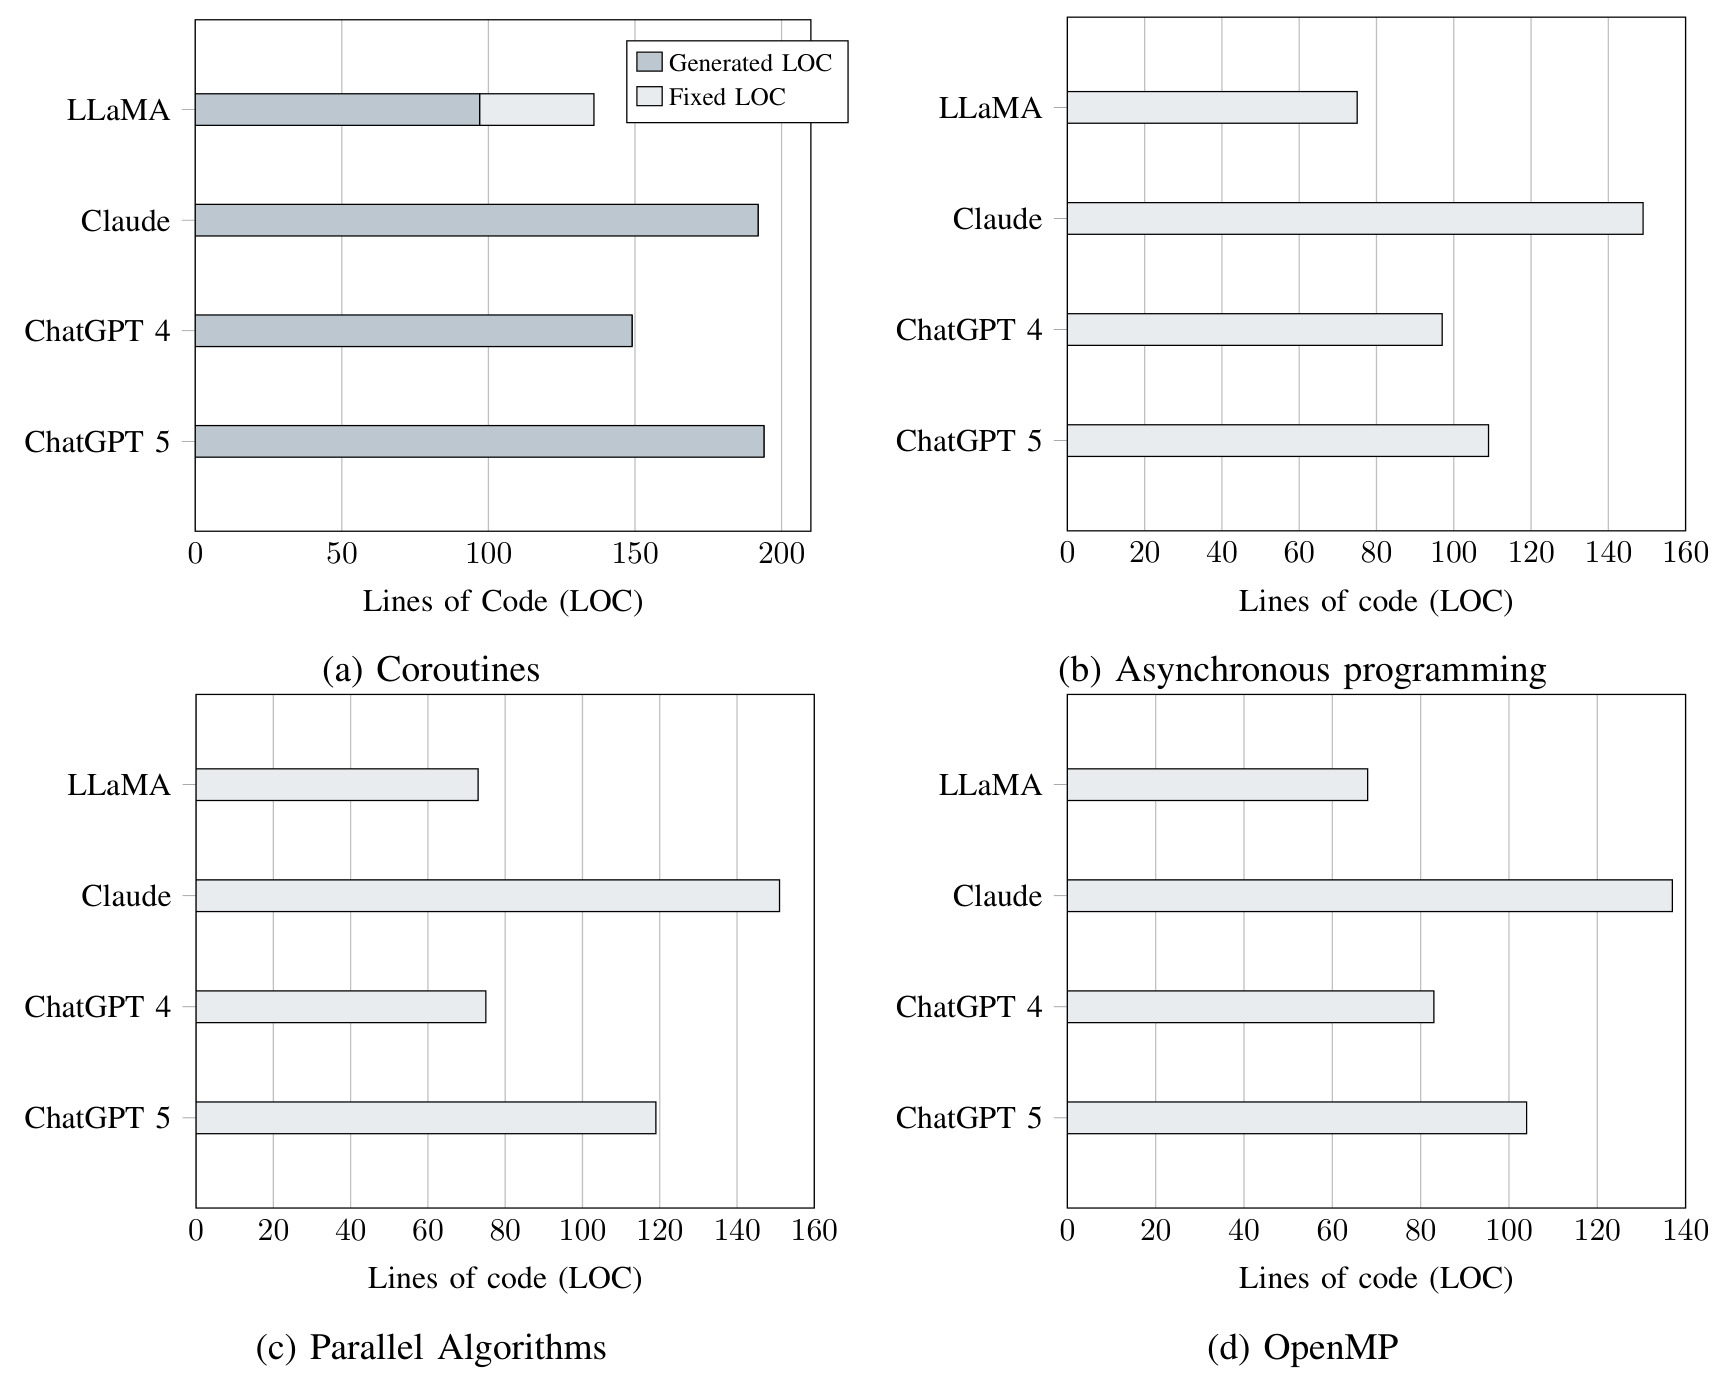
\includegraphics[width=0.92\linewidth]{fig_loc.png}\\[-1pt]
    {\tiny\color{Muted}Hình 3: LOC 4 biến thể chia sẻ (LLaMA coroutine phải thêm 37--39 dòng).}
  \end{column}
  \begin{column}{0.39\textwidth}
    \begin{bluebox}{MPI LOC (Bảng 9)}
      \centering
      \footnotesize
      \renewcommand{\arraystretch}{1.28}
      \begin{tabular}{@{}cccc@{}}
        \toprule
        \textbf{GPT-5} & \textbf{GPT-4} & \textbf{Claude} & \textbf{LLaMA} \\
        \midrule
        143 & 91 & 116 & 71 $\to$ \warn{82} \\
        \bottomrule
      \end{tabular}
      \vspace{0.22cm}
      \raggedright
      \begin{itemize}\footnotesize\setlength{\itemsep}{3pt}
        \item LLaMA ngắn nhất nhưng phải \textbf{vá thêm 37--39 dòng} ở coroutine và 11 dòng ở MPI.
        \item GPT-5 dài nhất (143) nhưng \ok{sạch nhất}.
        \item Claude viết dài ở bộ nhớ chia sẻ nhưng vẫn treo coroutine.
      \end{itemize}
    \end{bluebox}
  \end{column}
\end{columns}
\end{frame}

% SLIDE 15: ĐÁNH GIÁ CHẤT LƯỢNG – CÔNG SỨC (COCOMO)
\begin{frame}{Đánh giá chất lượng -- công sức (COCOMO)}
\centering
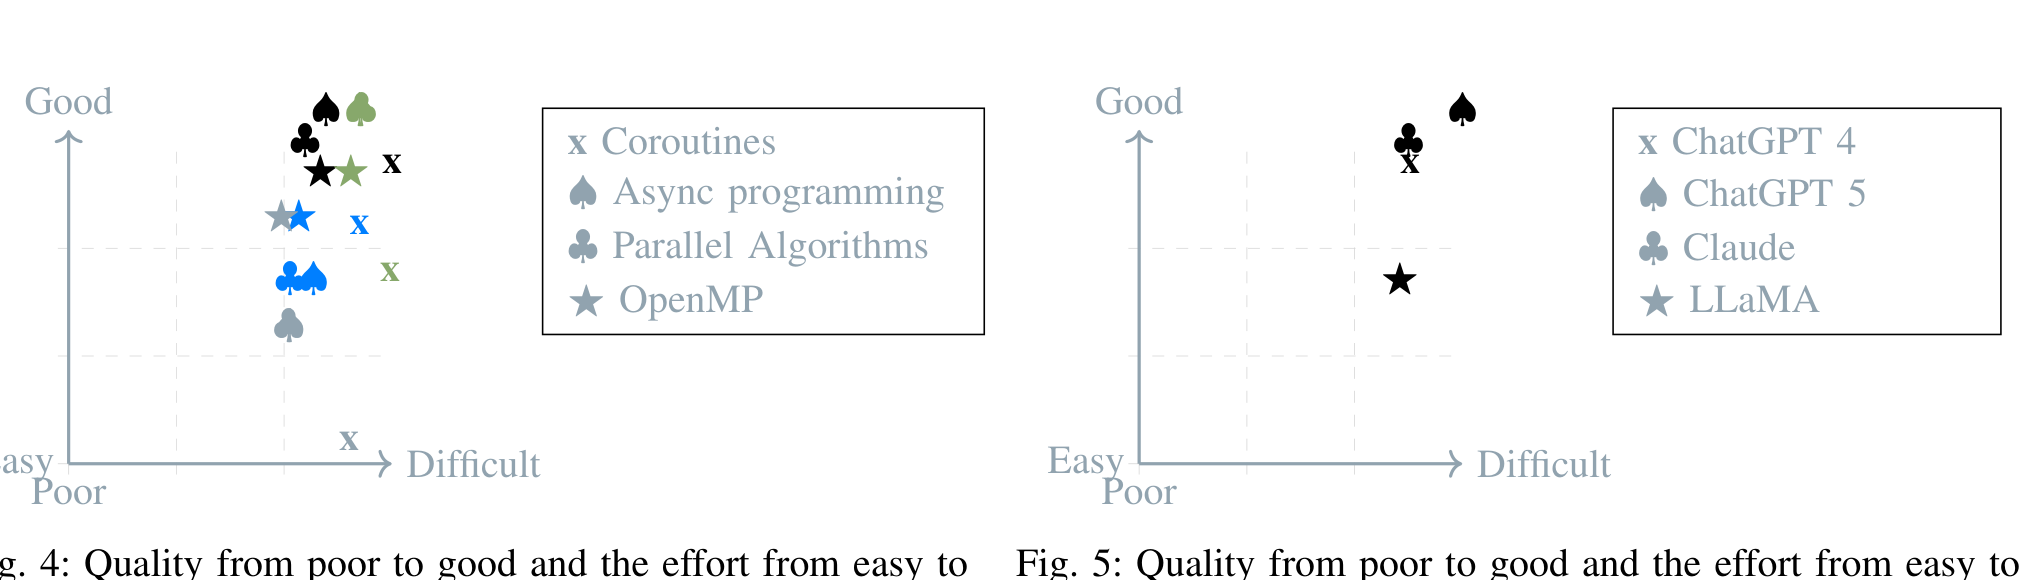
\includegraphics[width=0.92\textwidth]{fig_cocomo.png}\\[2pt]
{\scriptsize\color{Muted}Hình 4: Chất lượng (Poor $\to$ Good) vs Công sức COCOMO (Easy $\to$ Difficult).}

\vspace{0.35cm}
\begin{bluebox}[top=5pt,bottom=5pt]{Cách đọc Hình 4 \& Nhận xét}
  \begin{itemize}\footnotesize\setlength{\itemsep}{3.5pt}
    \item \textbf{Trái (chia sẻ):} màu = LLM (\textbf{Đen} GPT-5, \textcolor{BlueMid}{Xanh dương} GPT-4, \textcolor{OkGreen}{Xanh lá} Claude, \textcolor{Muted}{Xám} LLaMA); GPT-5 ở góc tốt, 2 \emph{outlier} LLaMA (xám) rơi xuống đáy.
    \item \textbf{Phải (MPI):} GPT-5 ($\spadesuit$) cao nhất; LLaMA ($\bigstar$) thấp nhất $\implies$ \textbf{chất lượng không tỉ lệ với LOC}.
  \end{itemize}
\end{bluebox}
\end{frame}

% ==========================================================================
% PHẦN 4: HIỆU NĂNG & TỔNG KẾT (NGUYỄN NHƯ BẢO)
% ==========================================================================
\setpart{Phần 4 \textbullet{} Nguyễn Như Bảo}

% SLIDE 16: MỞ RỘNG TRÊN 1 NÚT (HÌNH 5 — TOÀN CỠ, KHÔNG ĐÈ NHAU)
\begin{frame}{Khả năng mở rộng trên 1 nút (1--20 lõi, \texttt{pixel updates/s})}
\centering
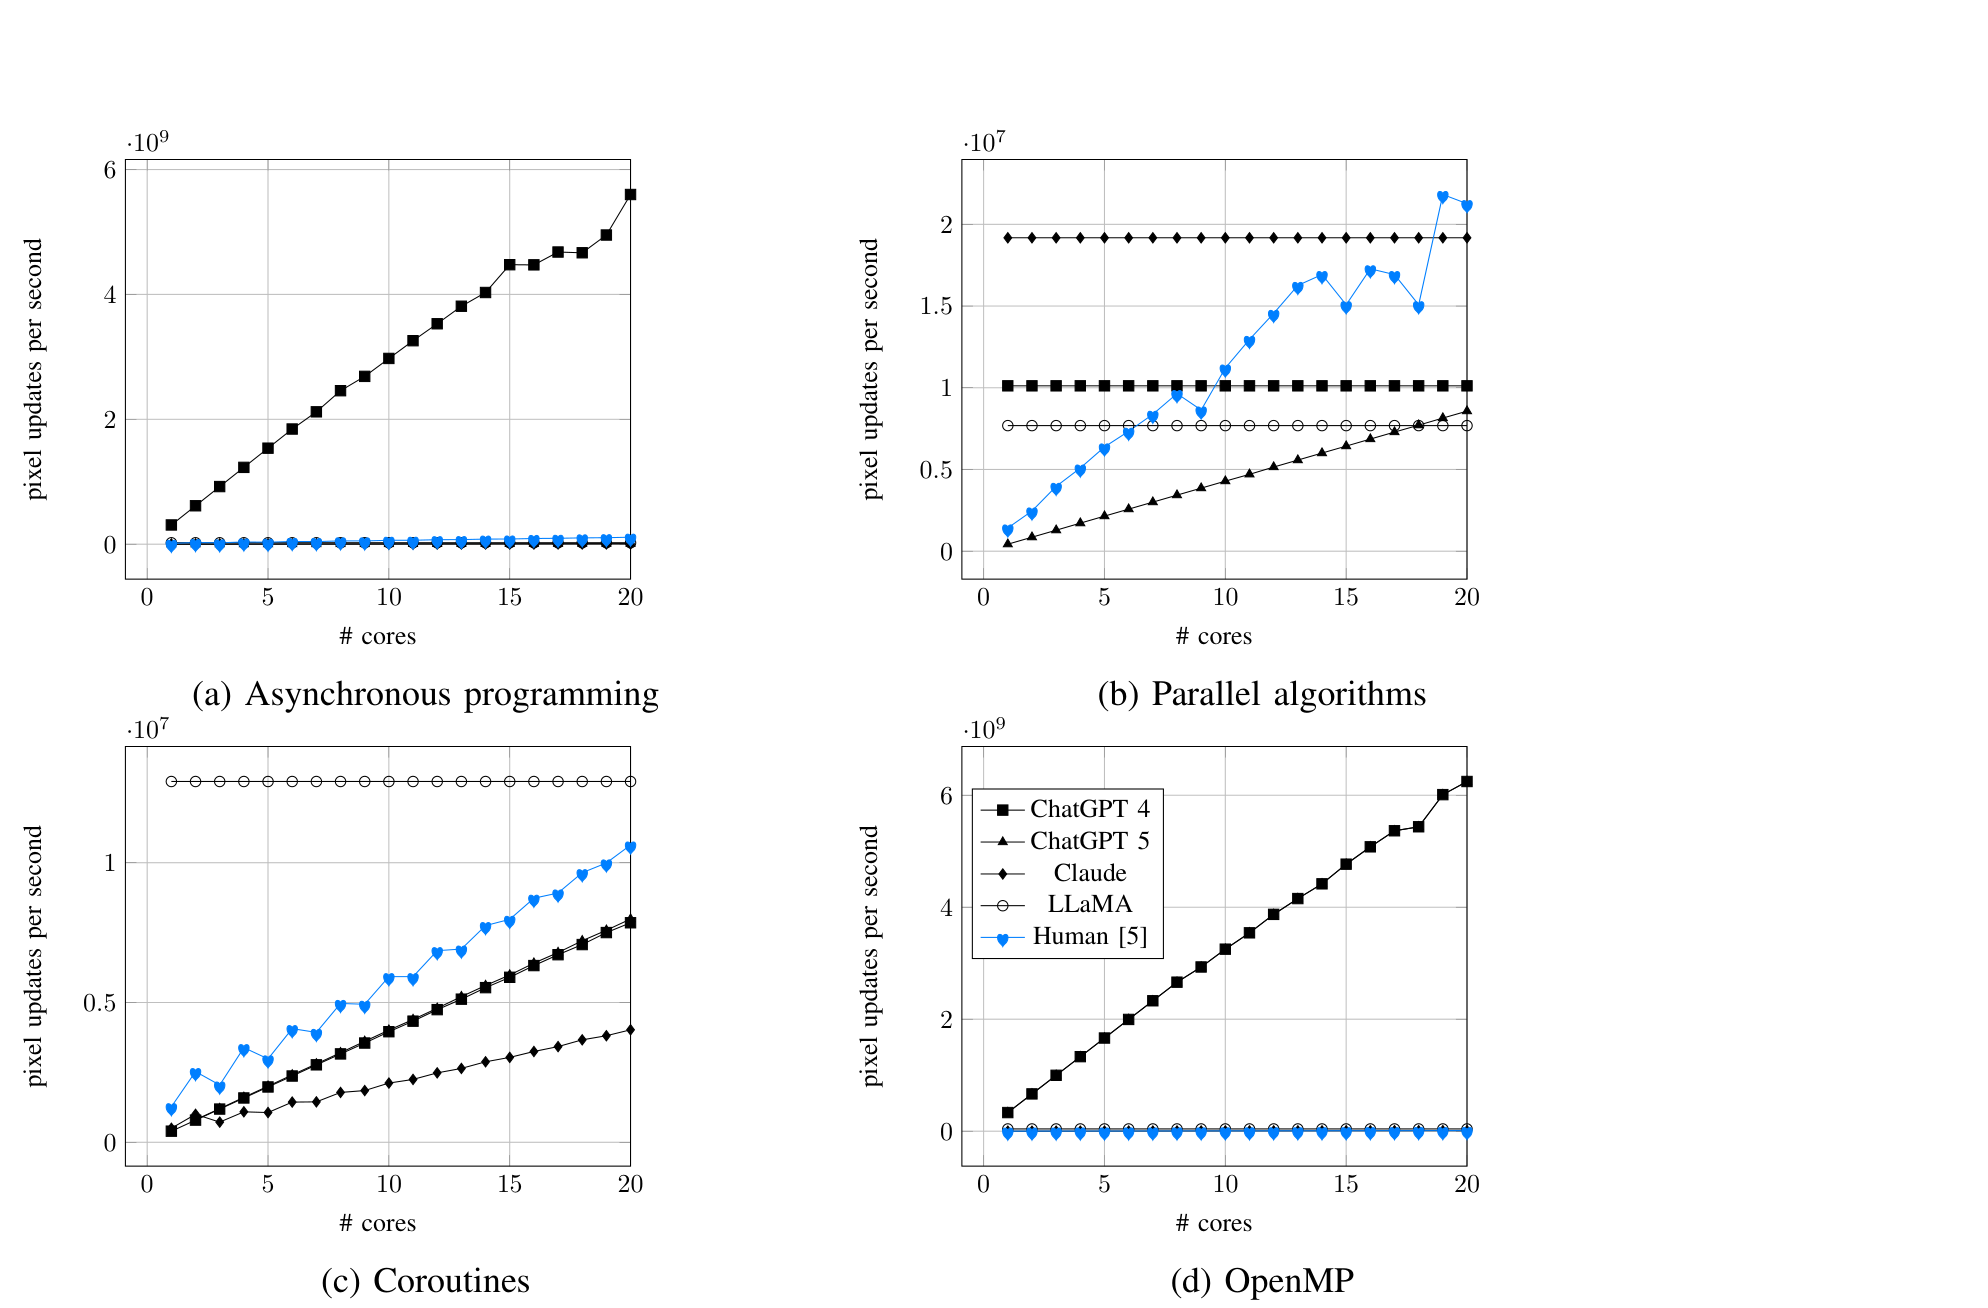
\includegraphics[height=6.25cm,trim=0.40cm 0.10cm 13.10cm 3.10cm,clip]{fig_scaling_shared.png}\\[2pt]
{\tiny\color{Muted}Hình 5: Mở rộng 1 nút (Xeon Gold 6148, 20 lõi). Chú ý: (a,d) thang $\times 10^9$, (b,c) thang $\times 10^7$; đường phẳng nằm \textbf{cao} = lỗi bỏ qua \code{-t}, đường sát trục 0 = bị nén thang đo.}
\end{frame}

% SLIDE 17: MỞ RỘNG PHÂN TÁN & SO SÁNH MÃ CON NGƯỜI
\begin{frame}{Mở rộng phân tán (1--12 nút) \& So sánh với mã con người}
\begin{columns}[T,totalwidth=\textwidth]
  \begin{column}{0.45\textwidth}
    {\footnotesize\bfseries\color{BlueDark}Hình 6: MPI+OpenMP (thang $\log_2$)}\vspace{3pt}
    \centering
    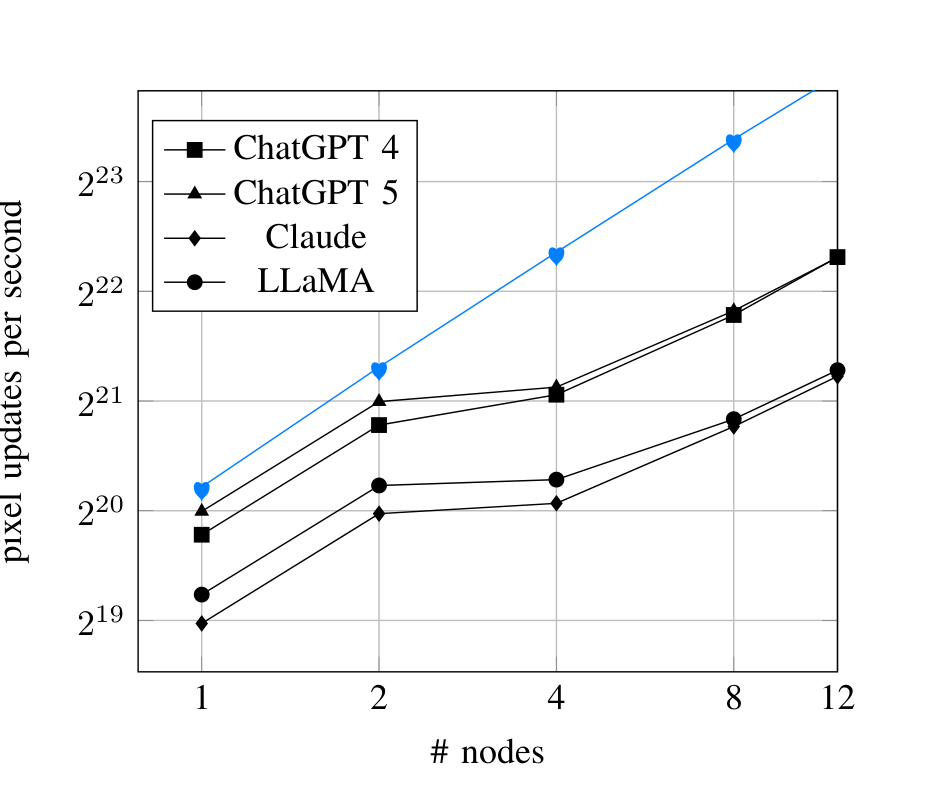
\includegraphics[width=0.73\linewidth,trim=0cm 0.3cm 1.4cm 1.5cm,clip]{fig_scaling_dist.png}\\[-1pt]
    {\tiny\color{Muted}Đường xanh trái tim là \code{Human [5]}.}
    \vspace{0.18cm}
    \begin{bluebox}[height=1.34cm,top=3pt,bottom=3pt]{Vì sao chững ở $2\to 4$ nút?}
      \scriptsize Chia 4 dải thì \textbf{2 dải giữa ôm ruột đen} $\implies$ chặn bước \code{MPI\_Gather}.
    \end{bluebox}
  \end{column}
  \begin{column}{0.52\textwidth}
    \begin{bluebox}[height=4.74cm,top=5pt,bottom=5pt]{Bảng 10: So sánh mã sách \emph{Parallel C++} (\texttt{Human [5]})}
      \scriptsize
      \renewcommand{\arraystretch}{1.38}
      \begin{tabularx}{\textwidth}{@{}>{\bfseries\color{BlueDark}}l >{\raggedright\arraybackslash}X >{\raggedright\arraybackslash}l@{}}
        \toprule
        \textbf{Biến thể} & \textbf{Kết quả} & \textbf{Nhận xét} \\
        \midrule
        Async      & GPT-4 $>$ mã sách      & Mẫu quen \\
        Par\_algo  & Sách $> 2\times$ GPT-5 & Mở rộng tốt \\
        Coroutine  & Sách $>$ GPT-4/5       & Cách biệt lớn \\
        OpenMP     & GPT-5 $>$ mã sách      & Ngoại lệ \\
        MPI+OpenMP & Sách dẫn đầu           & Phân vùng tốt \\
        \bottomrule
      \end{tabularx}
    \end{bluebox}
    \vspace{0.20cm}
    \begin{hboxcard}[height=1.34cm,top=3pt,bottom=3pt]{Kết luận so sánh}
      \scriptsize LLM thắng mẫu quen (async, OpenMP), \textbf{thua mẫu điều phối} (TBB, coroutine, MPI).
    \end{hboxcard}
  \end{column}
\end{columns}
\end{frame}

% SLIDE 17: BỔ SUNG THỰC NGHIỆM GEMINI 4 HYDROGEN (ẢNH & BẢNG 11)
\begin{frame}{Bổ sung thực nghiệm: Kiểm chứng Gemini 4 Hydrogen (Mục 4.9)}
\begin{columns}[T,totalwidth=\textwidth]
  \begin{column}{0.42\textwidth}
    \centering
    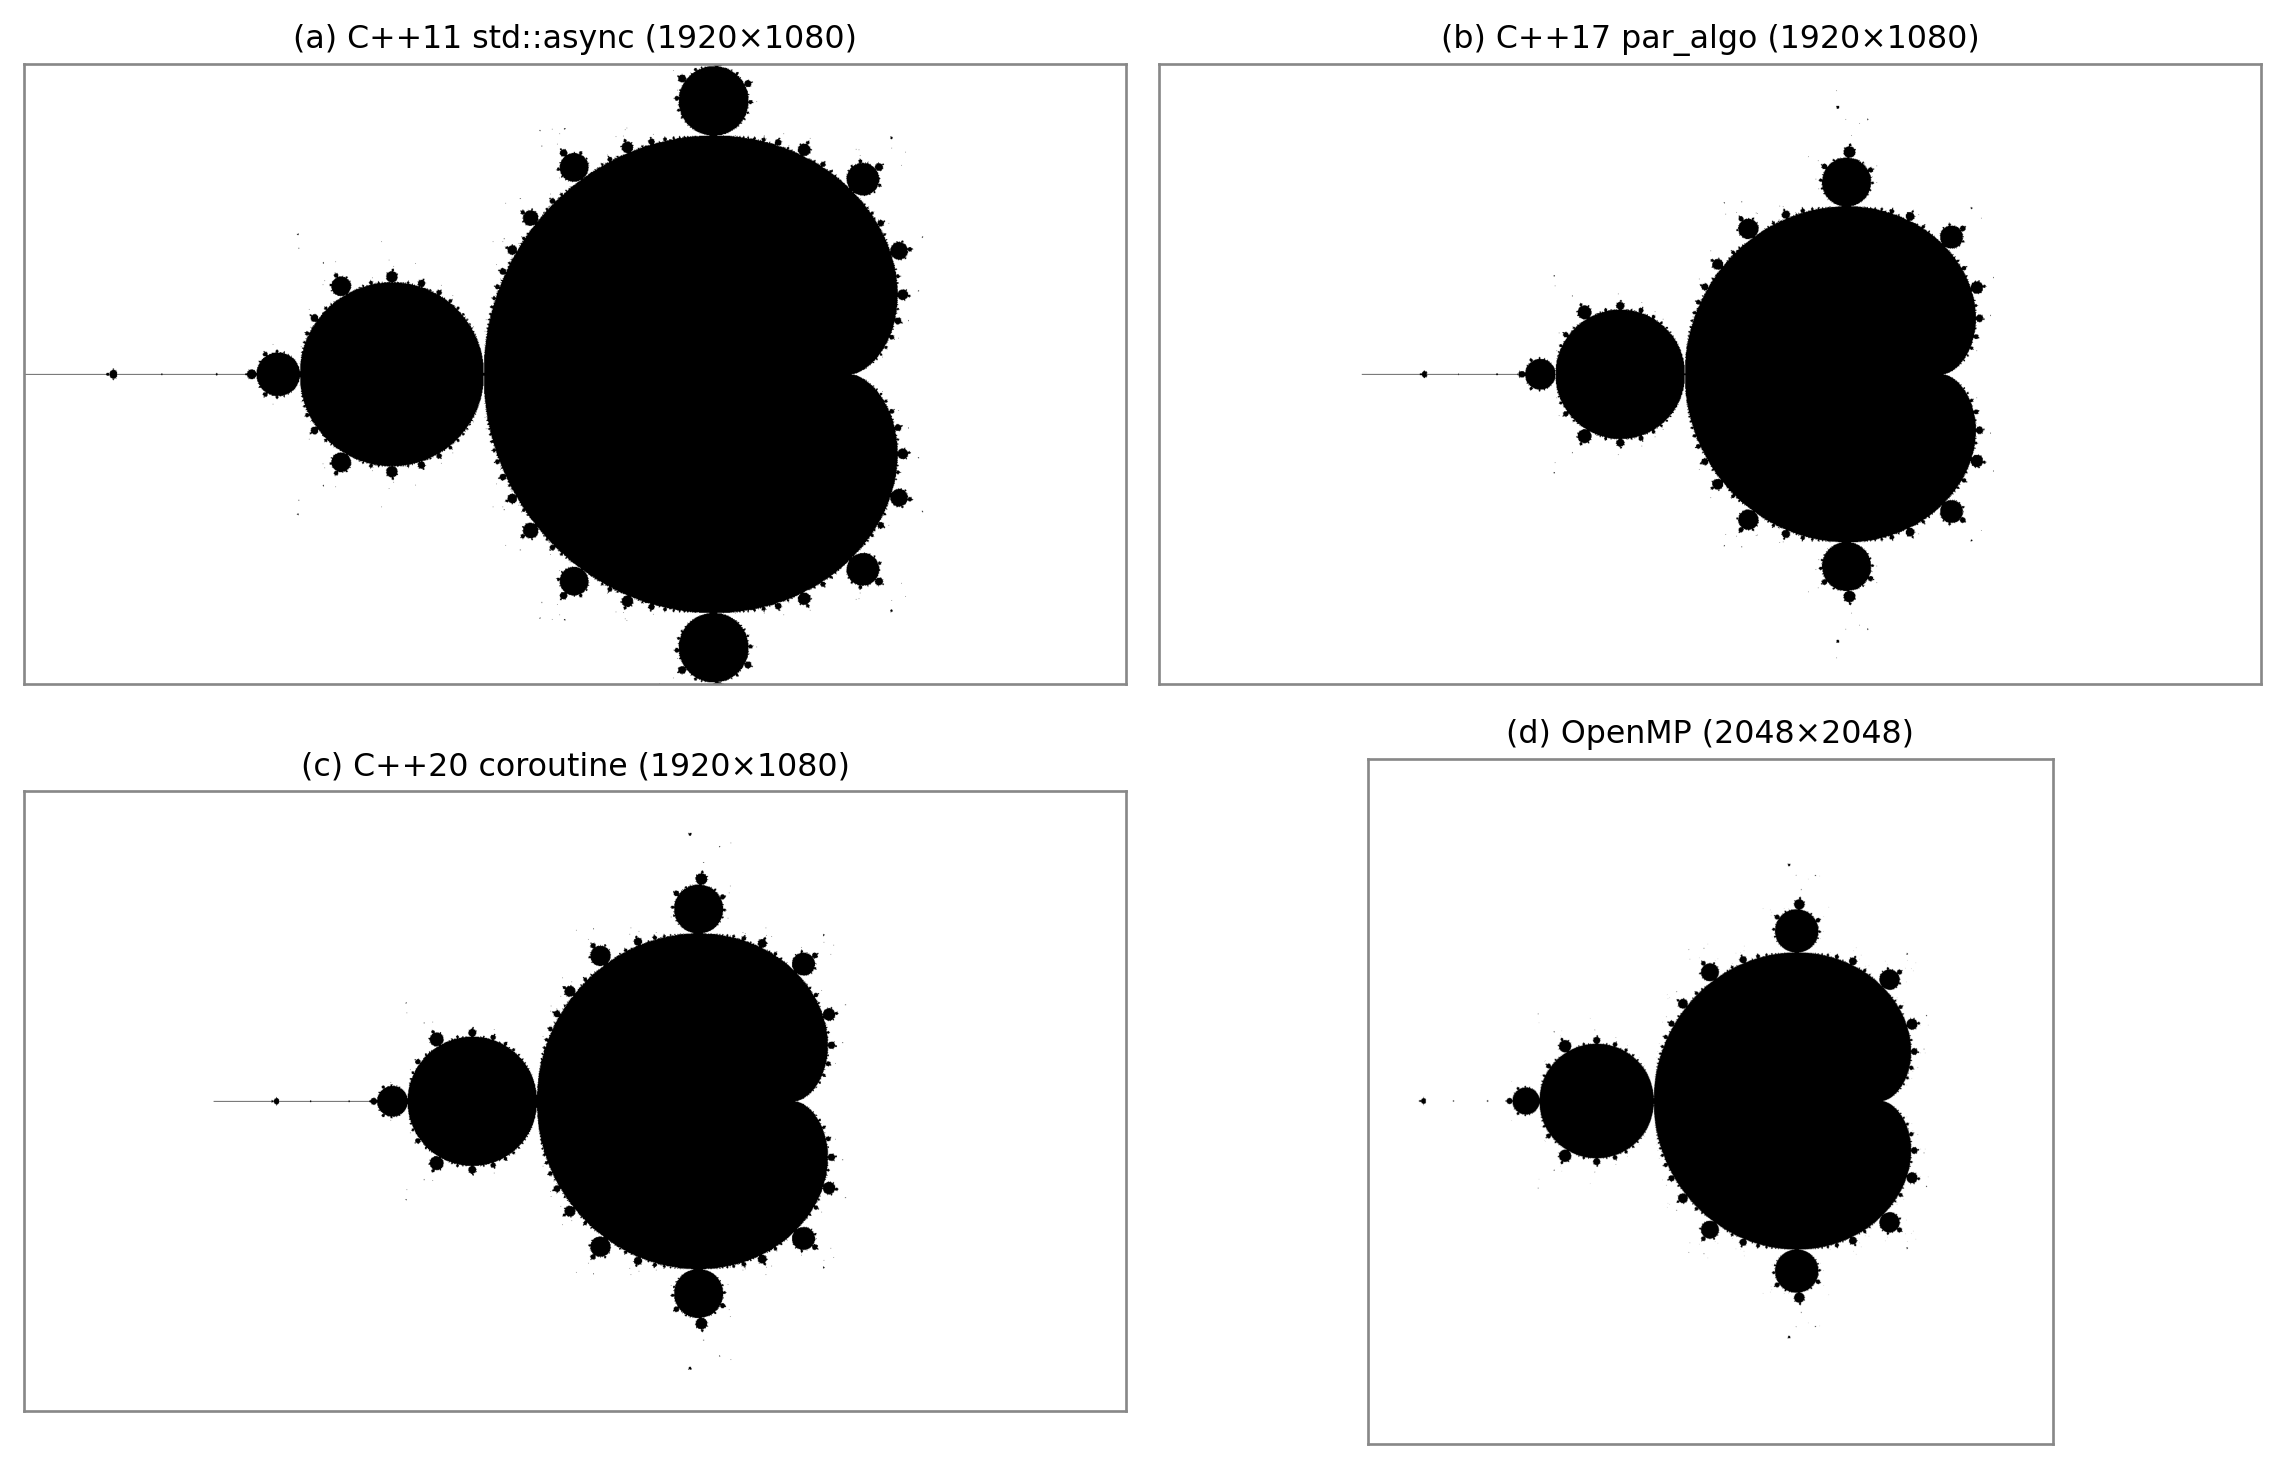
\includegraphics[width=0.94\linewidth]{fig_gemini4_mandelbrot.png}\\[-1pt]
    {\tiny\color{Muted}Hình 7: 4 ảnh P4 hợp lệ sinh ngay lần đầu (0 lỗi ảnh đen P4/P5).}
    \vspace{0.34cm}
    \begin{hboxcard}[height=1.82cm,top=3pt,bottom=3pt]{Thiết lập cục bộ (tách biệt cụm \texttt{rostam})}
      \scriptsize Windows 11, 12 luồng, GCC 13.2.0, nguyên văn P1--P3, mã \textbf{lần sinh đầu (0 chỉnh sửa)}. Kết quả chỉ dùng so sánh xu hướng mở rộng, không gộp trực tiếp vào Bảng 6.
    \end{hboxcard}
  \end{column}
  \begin{column}{0.56\textwidth}
    {\footnotesize\bfseries\color{BlueDark}Bảng 11: Kết quả mã nguyên bản Gemini 4 (Effort: High)}\vspace{2pt}
    \scriptsize
    \setlength{\tabcolsep}{3.5pt}
    \renewcommand{\arraystretch}{1.16}
    \begin{tabularx}{\textwidth}{@{}>{\bfseries\color{BlueDark}}l r c c c >{\raggedright\arraybackslash}X@{}}
      \toprule
      \rowcolor{BlueSoft}
      \textbf{Biến thể} & \textbf{LOC} & \textbf{Build} & \textbf{px/s$^\dagger$} & \textbf{Spd.} & \textbf{Điểm nổi bật} \\
      \midrule
      C++11 async & 133 & \ok{\checkmark\,(0)} & 1,75 & \ok{10,56$\times$} & Hàng đợi động \code{atomic} \\
      C++17 par\_algo & 163 & \ok{\checkmark\,(0)$^*$} & 2,98$^*$ & 1,02$\times^*$ & Kiểm tra TBB + cắt tỉa \\
      C++20 coroutine & 205 & \ok{\checkmark\,(0)} & 1,85 & \ok{10,50$\times$} & \code{jthread} + \code{latch}, hết treo \\
      OpenMP & 100 & \ok{\checkmark\,(0)} & \ok{3,23} & \ok{11,23$\times$} & \code{dynamic}, ảnh $2048^2$ \\
      MPI+OpenMP & 199 & -- & -- & -- & Tĩnh đạt: \emph{block-cyclic}, \code{Gatherv} \\
      \bottomrule
    \end{tabularx}
    \vspace{1pt}
    {\tiny\color{Muted}$^\dagger$ Đơn vị $\times 10^7$ px/s tại \code{-t 12}. $^*$ Không TBB chạy tuần tự ($2{,}91\times 10^7$ px/s nhờ cắt tỉa hình tim + bóng chu kỳ 2).}
    \vspace{3pt}
    \begin{bluebox}[height=1.82cm,top=3pt,bottom=3pt]{Bước tiến rõ rệt so với thế hệ 2025}
      \scriptsize Khắc phục triệt để lỗi treo coroutine \code{done()}, nhầm TBB/OpenMP, ảnh đen P4/P5 và đặt sai mốc đo MPI; chỉ còn chi tiết nhỏ (thiếu \code{<algorithm>} tường minh ở OpenMP, cờ \code{-i}/\code{-m} lệch tên).
    \end{bluebox}
  \end{column}
\end{columns}
\end{frame}

% SLIDE 18: THÔNG LƯỢNG GEMINI 4 CÙNG HỆ QUY CHIẾU (HÌNH 8)
\begin{frame}{Mở rộng 1 nút của Gemini 4 theo hệ quy chiếu \texttt{pixel updates/s}}
\centering
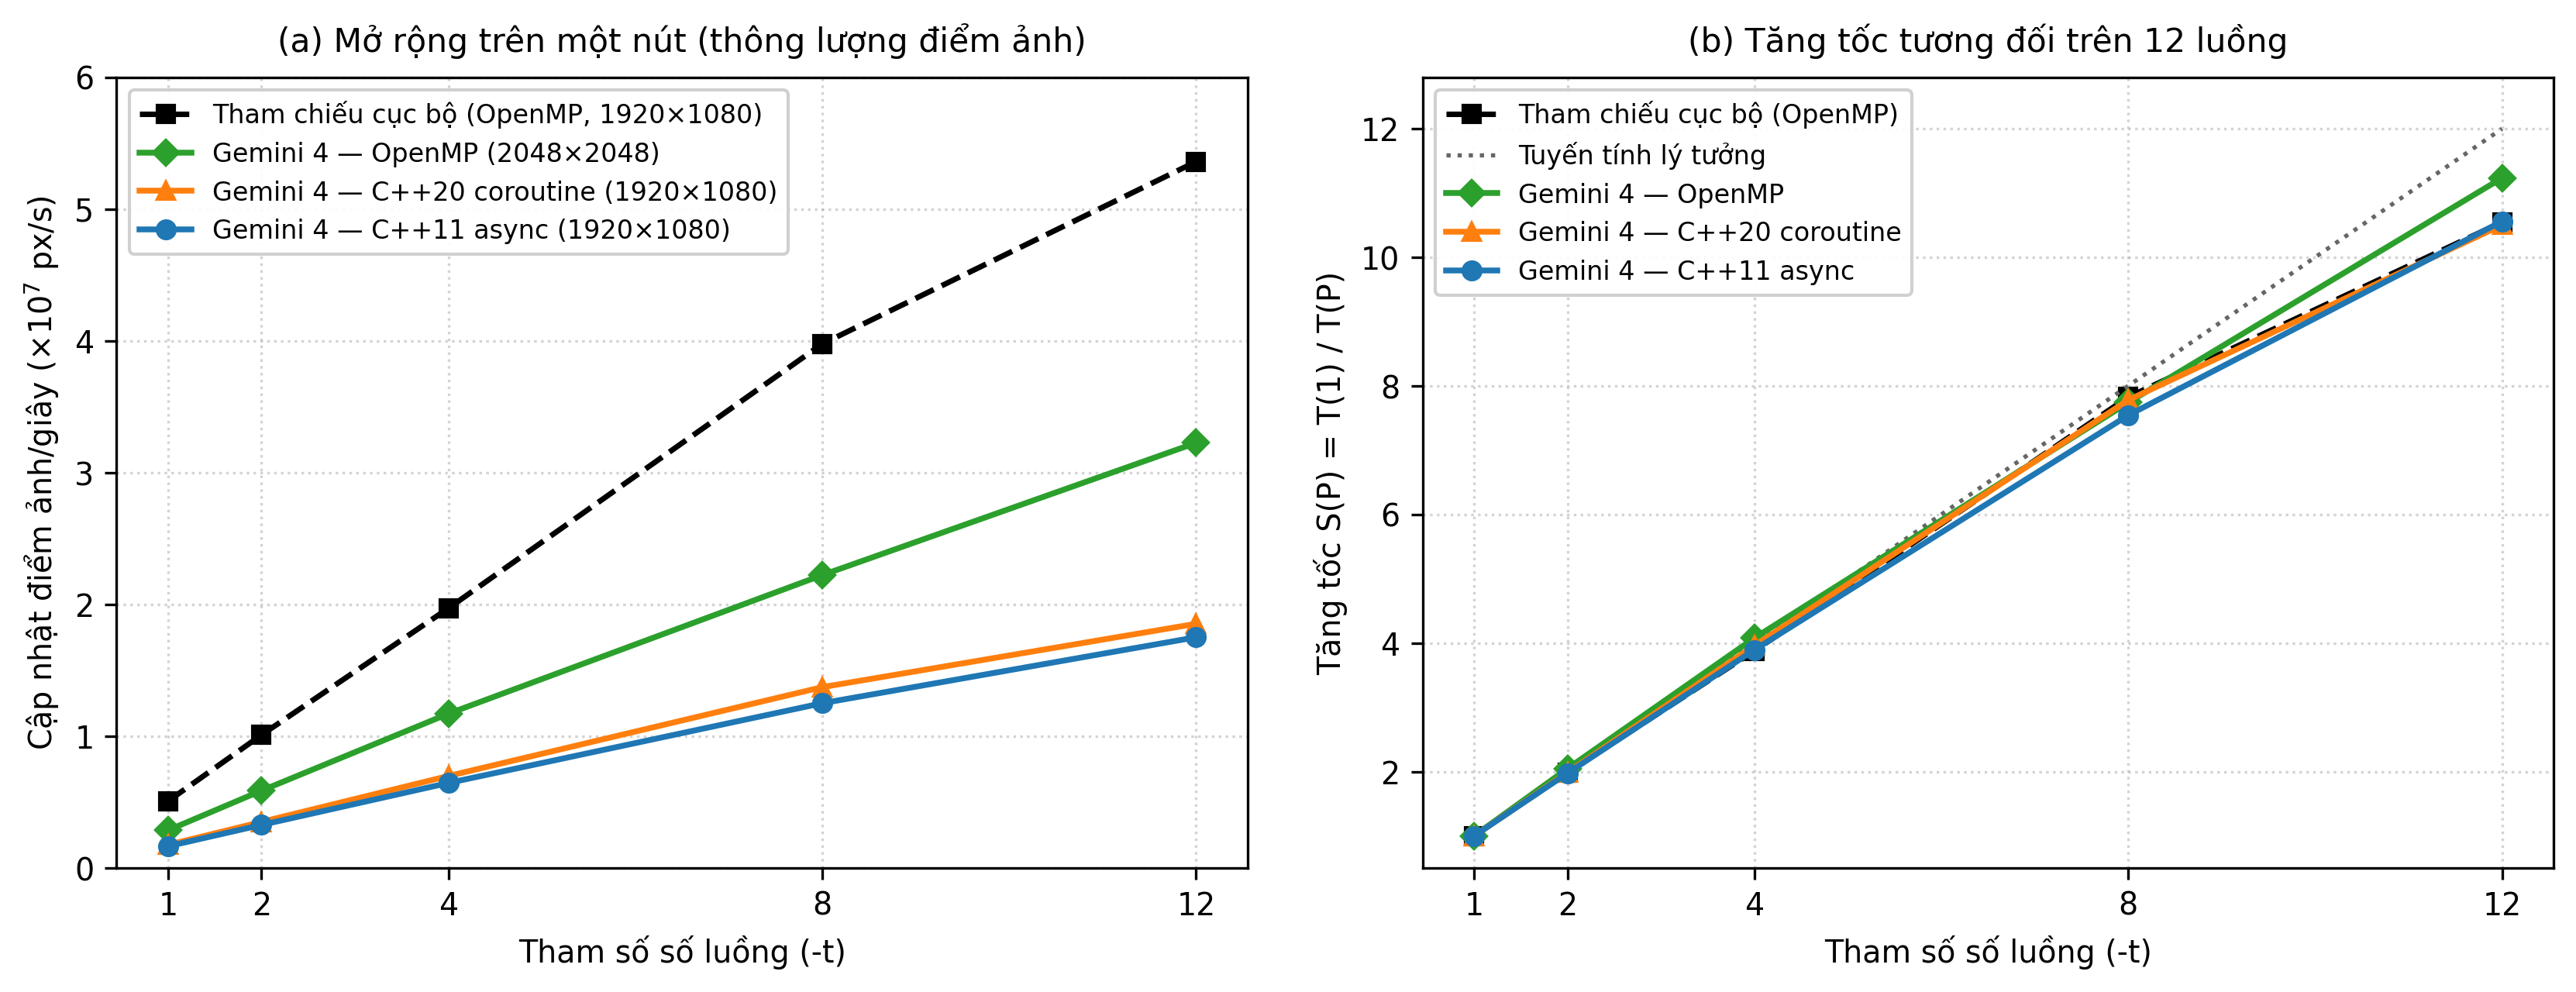
\includegraphics[width=0.70\textwidth]{fig_gemini4_scaling.png}\\[-2pt]
{\tiny\color{Muted}Hình 8: Thông lượng ($\times 10^7$ px/s --- cùng hệ quy chiếu Hình 5) và tăng tốc tương đối trên 12 luồng cục bộ (trung bình 3 lần đo, loại I/O).}

\vspace{0.16cm}
\begin{columns}[T,totalwidth=\textwidth]
  \begin{column}{0.32\textwidth}
    \begin{bluebox}[height=2.45cm,top=3pt,bottom=3pt]{1. Mở rộng tuyến tính sạch}
      \scriptsize Cả 3 biến thể tôn trọng \code{-t}, bám sát hoặc nhỉnh hơn mốc \code{mandel\_omp} ($10{,}55\times$): OpenMP đạt \ok{11,23$\times$}, async \ok{10,56$\times$}, coroutine \ok{10,50$\times$}.
    \end{bluebox}
  \end{column}
  \begin{column}{0.32\textwidth}
    \begin{bluebox}[height=2.45cm,top=3pt,bottom=3pt]{2. Đưa về \texttt{px/s} rất quan trọng}
      \scriptsize Theo giây, \code{openmp.cpp} ($0{,}130$\,s) có vẻ chậm hơn \code{coroutine} ($0{,}112$\,s); quy về \code{px/s}, OpenMP dẫn đầu (\ok{3,23$\times 10^7$}) vì xử lý ảnh $2048^2$ (gấp đôi pixel).
    \end{bluebox}
  \end{column}
  \begin{column}{0.32\textwidth}
    \begin{bluebox}[height=2.45cm,top=3pt,bottom=3pt]{3. Ảnh hưởng khung tọa độ}
      \scriptsize Mốc \code{mandel\_omp} ($5{,}36\times 10^7$) cao hơn vì diện tích miền phức rộng \textbf{16,0} (thoát sớm) so với \textbf{9,0} (OpenMP) và \textbf{5,06} (async) $\implies$ cần cố định tọa độ trong prompt!
    \end{bluebox}
  \end{column}
\end{columns}
\end{frame}

% SLIDE 19: KẾT LUẬN, KHUYẾN NGHỊ & HƯỚNG PHÁT TRIỂN
\begin{frame}{Kết luận, 5 khuyến nghị thực hành \& Hướng phát triển}
\begin{columns}[T,totalwidth=\textwidth]
  \begin{column}{0.52\textwidth}
    \begin{bluebox}[height=5.90cm]{5 khuyến nghị thực dụng khi dùng LLM cho HPC}
      \begin{enumerate}\scriptsize\setlength{\itemsep}{4pt}
        \item \textbf{Coi mã LLM là bản nháp:} luôn bật \code{-Wall -Wextra}, test dữ liệu nhỏ và kiểm tra đầu ra.
        \item \textbf{Đo mở rộng thay vì tin vào cờ \code{-t}:} xác minh backend thực tế (TBB vs OpenMP) bằng phép đo.
        \item \textbf{Soát kỹ Coroutine \& MPI:} kiểm tra \code{final\_suspend}, quyền sở hữu frame, \code{MPI\_Gatherv} và mốc timer đặt sau gather.
        \item \textbf{Kiểm tra định dạng dữ liệu:} kiểm tra header \code{P4/P5}, kích thước tệp và mở ảnh trực quan.
        \item \textbf{Prompt nêu rõ ràng buộc phi chức năng:} độ phân giải, tọa độ phức, chuẩn C++, loại trừ I/O và yêu cầu chia việc.
      \end{enumerate}
    \end{bluebox}
  \end{column}
  \begin{column}{0.45\textwidth}
    \begin{hboxcard}[height=1.95cm]{Kết luận trung tâm}
      \scriptsize LLM là \textbf{trợ lý sinh bản nháp HPC rất hiệu quả} (thế hệ 2026 như Gemini 4 tiến bộ mạnh), nhưng \textbf{chưa thay thế kỹ sư HPC} ở khâu kiểm duyệt ngữ cảnh thực thi \& tối ưu.
    \end{hboxcard}
    \vspace{0.20cm}
    \begin{bluebox}[height=3.75cm]{Hạn chế \& 4 hướng phát triển}
      \begin{itemize}\scriptsize\setlength{\itemsep}{2pt}
        \item \textbf{Hạn chế gốc:} sinh 1 lần, bài toán độc lập dữ liệu, 1 toolchain GCC.
        \item \textbf{Bài toán khó hơn:} stencil trao đổi halo, FFT song song, FEM.
        \item \textbf{Đánh giá thống kê \& Agentic:} lặp nhiều lần sinh, vòng lặp tự biên dịch--sửa lỗi (bối cảnh 3 công trình 2026 [9]--[11] trong báo cáo).
        \item \textbf{Tiêu chí mới:} vượt qua tỉ lệ biên dịch để chấm scaling \& chi phí bảo trì.
      \end{itemize}
    \end{bluebox}
  \end{column}
\end{columns}
\end{frame}

% ==========================================================================
% SLIDE 20: CẢM ƠN & HỎI ĐÁP (Q&A)
% ==========================================================================
\begin{frame}[plain]
\begin{tikzpicture}[remember picture,overlay]
  \fill[BlueDark] (current page.north west) rectangle (current page.south east);
  \fill[BlueMid] ([yshift=1.28cm]current page.south west) rectangle ([yshift=1.42cm]current page.south east);
  \fill[BlueMid,opacity=0.22] ([xshift=-5.2cm]current page.north east) -- (current page.north east) -- (current page.south east) -- cycle;

  \node[anchor=center,text=white,align=center] at ([yshift=0.85cm]current page.center) {%
    {\Huge\bfseries XIN CẢM ƠN THẦY VÀ CÁC BẠN!}\\[10pt]
    {\large\color{BlueSoft}Hỏi -- Đáp \& Trao đổi phản biện (Q\&A)}\\[18pt]
    \begin{minipage}{14.2cm}
      \centering
      \setlength{\tabcolsep}{4pt}
      \begin{tabular}{@{}p{3.35cm}p{3.35cm}p{3.35cm}p{3.35cm}@{}}
        \begin{tcolorbox}[colback=BlueMid!55!BlueDark,colframe=BlueBorder,boxrule=0.5pt,arc=2.5pt,height=1.22cm,valign=center,left=3pt,right=3pt,top=2pt,bottom=2pt,halign=center]
          {\scriptsize\bfseries\color{white}Trần Lý Dũng}\\[1pt]
          {\tiny\color{white!82}Phần 1: Giới thiệu bài toán}
        \end{tcolorbox} &
        \begin{tcolorbox}[colback=BlueMid!55!BlueDark,colframe=BlueBorder,boxrule=0.5pt,arc=2.5pt,height=1.22cm,valign=center,left=3pt,right=3pt,top=2pt,bottom=2pt,halign=center]
          {\scriptsize\bfseries\color{white}Nguyễn Quang Anh}\\[1pt]
          {\tiny\color{white!82}Phần 2: Thực nghiệm \& Demo}
        \end{tcolorbox} &
        \begin{tcolorbox}[colback=BlueMid!55!BlueDark,colframe=BlueBorder,boxrule=0.5pt,arc=2.5pt,height=1.22cm,valign=center,left=3pt,right=3pt,top=2pt,bottom=2pt,halign=center]
          {\scriptsize\bfseries\color{white}Đồng Đức Dương}\\[1pt]
          {\tiny\color{white!82}Phần 3: Phân tích lỗi thực tế}
        \end{tcolorbox} &
        \begin{tcolorbox}[colback=BlueMid!55!BlueDark,colframe=BlueBorder,boxrule=0.5pt,arc=2.5pt,height=1.22cm,valign=center,left=3pt,right=3pt,top=2pt,bottom=2pt,halign=center]
          {\scriptsize\bfseries\color{white}Nguyễn Như Bảo}\\[1pt]
          {\tiny\color{white!82}Phần 4: Hiệu năng \& Kết luận}
        \end{tcolorbox}
      \end{tabular}
    \end{minipage}
  };

  \node[anchor=south,text=white!80,font=\scriptsize] at ([yshift=0.42cm]current page.south) {%
    Báo cáo LaTeX \;\textbullet\; Demo Mandelbrot OpenMP (\texttt{\color{BlueSoft}Demo/interactive.py}) \;\textbullet\; Kiểm chứng Gemini 4 Hydrogen (\texttt{\color{BlueSoft}Demo/eval\_llm.py})
  };
\end{tikzpicture}
\end{frame}

\end{document}
